% MolDStruct SF/MD reference manual.  Build: tectonic manual.tex  (or pdflatex twice)
\documentclass[11pt,a4paper,openany]{report}
\usepackage[margin=2.5cm]{geometry}
\usepackage{amsmath,amssymb,bm}
\usepackage{booktabs,array,tabularx,longtable}
\usepackage{graphicx,caption}
\usepackage{xcolor}
\usepackage{float}
\usepackage{listings}
\usepackage{enumitem}
\usepackage[colorlinks=true,linkcolor=blue!50!black,citecolor=green!35!black,urlcolor=blue!50!black]{hyperref}

\definecolor{codebg}{RGB}{247,246,242}
\definecolor{codecomment}{RGB}{110,108,100}
\definecolor{devbox}{RGB}{252,243,228}
\lstset{basicstyle=\ttfamily\footnotesize, backgroundcolor=\color{codebg}, frame=single,
  rulecolor=\color{black!15}, framesep=4pt, xleftmargin=6pt, xrightmargin=6pt, columns=fullflexible,
  keepspaces=true, breaklines=true, showstringspaces=false, aboveskip=8pt, belowskip=8pt,
  commentstyle=\color{codecomment}\itshape}
\setlist{itemsep=2pt, topsep=4pt}
\emergencystretch=2em

\let\oldunderscore\_
\renewcommand{\_}{\oldunderscore\allowbreak}
\newcommand{\code}[1]{\texttt{#1}}
\newcommand{\opt}[1]{\texttt{#1}}            % an mdp option
\newcommand{\env}[1]{\texttt{#1}}            % an environment variable
\newcommand{\file}[1]{\texttt{#1}}
\newcommand{\dd}{\mathrm{d}}
\newcommand{\kc}{k_{\mathrm C}}
\newcommand{\Kmat}{\mathsf K}
\newcommand{\vect}[1]{\bm{#1}}
\newcommand{\devnote}[1]{\par\smallskip\noindent\colorbox{devbox}{\parbox{\dimexpr\linewidth-2\fboxsep}{\small
  \textbf{Development build.} #1}}\par\smallskip}

\title{\Huge MolDStruct SF/MD\\[8pt]
  \Large Strong-field (ADK) ionization and Coulomb explosion\\ with a trapped-electron cloud\\[18pt]
  \large Reference manual\\[14pt]
  \normalsize\itshape Disclaimer: This manual is AI-generated by claude opus 5.5 with human supervision based on notes,
  the source code, and simulation runs.\\[10pt]
  \normalsize\upshape The trapped-electron cloud (Chapters~\ref{ch:pb}--\ref{ch:coll}) is a \textbf{development build}
  (branch \code{pb-electrons}), not a release.}
\author{Biophysics group, Uppsala University}
\date{November 2026 \\[4pt] \small model version: tpr format 184}

\begin{document}
\maketitle
\tableofcontents

\chapter{Introduction}
\label{ch:intro}

MolDStruct SF/MD simulates what happens to a biomolecule, or any small system of light atoms, when it is hit by an
intense femtosecond \emph{optical} laser pulse.
The field of the pulse tears electrons out of the atoms by tunnelling, the sample charges up and explodes, and the
ions fly apart in directions that still carry information on the original structure.
The model follows the charge state of every atom, the electrons that are released, and the motion of the nuclei in one
simulation.

It is part of the MolDStruct toolbox and is built on GROMACS~4.5.4~\cite{pronk2013}, extended with an ionization
module.
Everything GROMACS does still works the same way; the ionization model is switched on with \code{mdrun -ionize} and
controlled by \opt{sfmd-*} options in the \file{.mdp} file.
Its sibling, MolDStruct MC/MD (\code{gromacs-mc}), treats X-ray pulses with a Monte Carlo of the inner-shell
processes; the two share the modified force field and, since November 2026, the trapped-electron cloud.

\section{The model in one page}

\begin{description}
  \item[Atoms] are classical particles with an integer charge.
    The charge is that of the ion's valence shell being stripped (H up to 1+, C 4+, N 5+, O 6+, S 6+), and it enters
    the force field.
  \item[The laser pulse] is a Gaussian in time with a carrier wave; its peak intensity follows from the pulse energy,
    duration and focal spot (Chapter~\ref{ch:adk}).
  \item[Tunnel ionization] is the Ammosov--Delone--Krainov (ADK) rate~\cite{adk1986,tong2002} of the instantaneous
    field for each atom's current charge state, turned into a probability per MD step and sampled (Chapter~\ref{ch:adk}).
  \item[The force field] is modified so that ionized atoms lose their chemical bonds: bonded terms fade out with the
    charge, bonds break irreversibly, and the Coulomb interactions between bonded neighbours are restored
    (Chapter~\ref{ch:ff}).
  \item[Released electrons] either escape or are trapped by the growing positive charge (optional,
    \opt{sfmd-electrons = pbgrid}).
    The trapped ones form a hot electron cloud, a continuous density in thermal equilibrium with the ions: a
    Poisson--Boltzmann problem solved on a three-dimensional grid every 0.2\,fs (Chapter~\ref{ch:pb}).
    The cloud screens the ions, pulls on them, decides which new electrons escape, and evaporates as the sample expands.
  \item[The laser acts on the cloud] by lowering its escape barrier and by heating it through inverse bremsstrahlung
    (Chapter~\ref{ch:laser}).
  \item[Electron--ion collisions] in the cloud ionize further, and after the pulse can recombine
    (Chapter~\ref{ch:coll}).
\end{description}

\section{When the cloud matters}

Without the cloud (\opt{sfmd-electrons = none}, the default) every electron leaves the instant it is freed, and the MD
sees bare ions.
For lysozyme (1960 atoms) at 850\,nm and 15\,fs that is a fair description at $10^{17}$\,W/cm$^2$, where the cloud is
gone before the pulse peak; at $10^{15}$\,W/cm$^2$ about half the electrons stay trapped, the ions reach only 0.3 of
their cloud-free kinetic energy, and the fast ions fly 6.5$^\circ$ away from their cloud-free directions
(Appendix~\ref{app:validation}).

\devnote{The cloud and everything built on it (the laser barrier and heating, impact ionization, recombination, the
temperature floor, long range, the direction autostop, the schedule) live on the \code{pb-electrons} branch of sf-md.
They were tested on lysozyme at $10^{15}$--$10^{17}$\,W/cm$^2$, 850\,nm, 15\,fs, but not yet against experiment or a
reference code; the results tables in Appendix~\ref{app:validation} are the evidence there is.}

\section{This manual}

Chapter~\ref{ch:start} gets a run going.
Chapters~\ref{ch:adk}--\ref{ch:coll} describe the physics, Chapter~\ref{ch:output} the output, and
Chapters~\ref{ch:mdp} and~\ref{ch:env} list every option and environment variable.
The appendices cover the numerics of the cloud, parallel runs, the tests behind the model, and version and compatibility
notes.
The code is in \file{src/kernel/sfionize.c} (ADK, the pulse, the run control) and \file{src/kernel/sfelectrons.c} (the
cloud), with the force field in \file{src/gmxlib/bondfree.c} and \file{nonbonded/nonbonded.c}.

\chapter{Getting started}
\label{ch:start}

\section{Building}

The build is that of GROMACS 4.5.4 with CMake; FFTW~3 in single precision is needed for the electron cloud.
From the source tree:
\begin{lstlisting}
cd gromacs-4.5.4-SFMD
mkdir build && cd build
cmake .. -DCMAKE_BUILD_TYPE=Release -DGMX_FFT_LIBRARY=fftw3 \
         -DCMAKE_INSTALL_PREFIX=/path/to/install
make -j8 install
\end{lstlisting}
For a reference build that must not change when libraries are rebuilt, add \code{-DBUILD\_SHARED\_LIBS=OFF}.
Run inputs must be written with this build's \code{grompp}: the \file{.tpr} carries the \opt{sfmd-*} options (format
185), which stock GROMACS and \code{gromacs-mc} cannot read.

\section{A first run}

\code{example/} is a complete run: lysozyme (PDB 1AKI, 1960 atoms) in vacuum, exploded by a 5\,mJ, 5\,fs pulse.
The steps are those of any GROMACS run, with \code{-ionize} added to \code{mdrun}:
\begin{lstlisting}
pdb2gmx -f 1aki.pdb -ff charmm27 -water none
grompp  -f exp.mdp -c conf.gro -p topol.top -o explode.tpr
mdrun   -deffnm explode -nt 4 -pd -ionize
\end{lstlisting}
\code{-water none} keeps \code{pdb2gmx} from asking; \code{-pd} (particle decomposition) is required for more than one
thread, because domain decomposition cannot follow an explosion (Appendix~\ref{app:parallel}).

The \file{.mdp} needs, besides the usual vacuum settings,
\begin{lstlisting}
dt                          = 0.000002   ; 2 as (ps!)
morse                       = yes        ; bonds that can break
pbc                         = no
coulombtype                 = Cut-off
sfmd-pulse-peak-time        = 35         ; fs
sfmd-pulse-fwhm             = 15         ; fs, full width at half maximum
sfmd-pulse-energy           = 1.13e-4    ; J
sfmd-pulse-focal-diameter   = 30000      ; nm
sfmd-pulse-wavelength       = 850        ; nm
\end{lstlisting}
Note the units: pulse times in fs, \code{dt} and \code{tinit} in GROMACS's ps.
These five pulse values give a peak intensity of $10^{15}$\,W/cm$^2$; the run summary prints it
(Section~\ref{sec:summaries}).
The cut-offs are set by \code{grompp} when the cloud is on (\opt{sfmd-pb-long-range = auto},
Section~\ref{sec:longrange}); without the cloud use \code{rcoulomb = rvdw = rlist = 0} (all pairs) or a cut-off that
covers the exploding sample.

\section{With the trapped-electron cloud}

\begin{lstlisting}
sfmd-electrons          = pbgrid
sfmd-coll-recombination = 2      ; optional: recombination after the pulse
\end{lstlisting}
With \opt{sfmd-electrons = pbgrid} the cloud's options default to the recommended model: the laser barrier, laser
heating of an ellipsoidal cloud with surface damping, electron-impact ionization and a 1\,eV temperature floor
(Chapters~\ref{ch:pb}--\ref{ch:coll}).
Each can be switched off on its own.
Recombination stays off by default; after the pulse (\opt{= 2}) it gives back most of the extra charge impact
ionization creates without changing the explosion.

\devnote{Before 11 November 2026 the cloud's options all defaulted to 0. An \file{.mdp} written then that relied on the
defaults now gets the full model; set the options to 0 (and \opt{sfmd-heating-shape = sphere}) to reproduce it. A
\file{.tpr} keeps what it was made with.}

\section{How long to run}

The ions' directions settle within roughly 100\,fs of the pulse; their kinetic energy keeps growing slowly much longer.
Two options cut the cost:
\begin{description}
  \item[\opt{sfmd-autostop = 2}] stops the run once the heavy-ion velocity directions have settled: every
    \opt{sfmd-autostop-interval} (5\,fs) the median turn since the last check is extrapolated as $1/(t-t_{\mathrm{peak}})^2$,
    and the run stops when the turn still to come is below \opt{sfmd-autostop-angle} (2$^\circ$), but not before
    \opt{sfmd-autostop-min-time} (60\,fs) after the pulse peak; \code{nsteps} stays the upper limit.
    On lysozyme it stopped at 95\,fs ($10^{16}$) and 125--130\,fs ($10^{15}$), with the directions still turning
    0.4--2.2$^\circ$ by 300\,fs against a seed spread of 1--5$^\circ$, and the ion energy 6\,\% short of its 300\,fs value;
    2.5--3.3$\times$ less wall time.
    \opt{sfmd-autostop = 1} is the older stop at a ratio of kinetic to total energy.
  \item[\opt{sfmd-schedule}] lengthens the step and the cloud-solve interval after the pulse, e.g.
    \code{65:0.01:0.2 95:0.1:2 135:0.1:5} (from 65\,fs a 10\,as step and a solve every 0.2\,fs, and so on).
    \code{nsteps} $\times$ \code{dt} stays the end time.
    \code{grompp} refuses a first change before the pulse peak + $3\sigma$ (changing the step while ADK still ionizes
    changes the run's random history) and output intervals the new steps do not divide.
    On lysozyme the schedule above moved the directions by at most 1.2$^\circ$ and the ion energy by $-0.2$\,\% at
    300\,fs, 2.8--3.1$\times$ faster.
    Off by default.
\end{description}
Compare kinetic energies only between runs stopped or scheduled the same way.

\section{Seeds and ensembles}
\label{sec:seeds}

The ADK draws are seeded from \code{/dev/random}, so every run is an independent realization --- what an ensemble
needs.
\env{GMX\_SFMD\_SEED=n} pins the seed; each rank still gets its own stream (the rank index is mixed in), so a pinned
run is reproducible for a given rank count only.
The seed used is in the run summary.
Fixed seeds are for tests, not for production ensembles.

\section{Chaining runs}

\opt{sfmd-initial-charges = 1} starts from the charges in \file{charges.txt} (atom index and charge per line), which a
finished run writes into \file{simulation\_output/}.
It cannot be used with the cloud, whose state is not saved; \code{grompp} refuses the combination.

\section{The run summary}

At the first step \code{mdrun} prints a summary of what the run will do --- system, pulse with its peak intensity and
field, length, schedule, seed, ranks, every process with its settings --- and warnings for settings outside what was
tested (Section~\ref{sec:summaries}).
Read it first.

\chapter{The laser pulse and tunnel ionization}
\label{ch:adk}

\section{The pulse}

The pulse is a linearly polarized Gaussian with a carrier wave,
\begin{equation}
  I(t) = I_0\,e^{-(t-t_0)^2/2\sigma^2},\qquad
  E(t) = E_0\,e^{-(t-t_0)^2/4\sigma^2}\cos\!\big(\omega(t-t_0)+\varphi\big),
\end{equation}
with $t_0$ = \opt{sfmd-pulse-peak-time}, $\sigma$ = \opt{sfmd-pulse-fwhm}$/2\sqrt{2\ln2}$, $\omega = 2\pi c/\lambda$
($\lambda$ = \opt{sfmd-pulse-wavelength}) and a carrier phase $\varphi$ drawn uniformly in $[-\pi/2,\pi/2]$ per run (and
broadcast, so that all ranks see the same field).
The peak intensity follows from the pulse energy $E_p$ = \opt{sfmd-pulse-energy} spread uniformly over a disc of diameter
$d$ = \opt{sfmd-pulse-focal-diameter}:
\begin{equation}
  I_0 = \frac{E_p}{\pi(d/2)^2\,\sigma\sqrt{2\pi}},\qquad E_0 = \sqrt{2I_0/(c\varepsilon_0)}.
\end{equation}
The sample (a few nm) is far smaller than the wavelength, so the field is uniform over it.
It has no direction in the model: ADK depends only on $|E(t)|$, and the cloud sees a cycle-averaged field
(Chapter~\ref{ch:laser}).
The field is evaluated within $\pm6\sigma$ of the peak and is zero outside; \file{pulse\_profile.txt} has $I(t)$ and
$E(t)$ every step.

\section{The ADK rate}

An atom in charge state $q$ is ionized to $q+1$ at the static-field tunnelling rate of Ammosov, Delone and
Krainov~\cite{adk1986}, in the form of Tong and Lin~\cite{tong2002} (atomic units):
\begin{gather}
  W = |C_{n^*l^*}|^2\,f(l,m)\,I_p\,\Big(\frac{2(2I_p)^{3/2}}{F}\Big)^{2n^*-|m|-1}
      \exp\!\Big(-\frac{2(2I_p)^{3/2}}{3F}\Big),\\
  |C_{n^*l^*}|^2 = \frac{1}{2\pi n^*}\Big(\frac{2e}{n^*}\Big)^{2n^*},\qquad
  f(l,m) = \frac{(2l+1)\,(l+|m|)!}{2^{|m|}\,|m|!\,(l-|m|)!},\qquad n^* = \frac{Z}{\sqrt{2I_p}},
\end{gather}
with $F = |E(t)|$ the instantaneous field, $I_p$ the ionization energy of the state, and $Z = q+1$ the charge left
behind.
The instantaneous (not cycle-averaged) rate is used, with the field of the current step, so ionization happens near the
field crests; at 2\,as there are $\sim$1400 steps per optical cycle at 850\,nm.
The constants of every state are computed once at start-up and printed to the \file{.log}.

\begin{table}[H]
\centering\small
\begin{tabular}{@{}l l l l@{}}
\toprule
element & ionization energies (eV), $q\to q+1$ & orbital ($n,l,|m|$) & states \\
\midrule
H & 13.598 & 1s & 1 \\
C & 11.260, 24.383, 47.887, 64.494 & 2p ($|m|$ 0, 1), then 2s & 4 \\
N & 14.534, 29.601, 47.448, 77.473, 97.890 & 2p ($|m|$ 0, 1, 1), then 2s & 5 \\
O & 13.618, 35.117, 54.936, 77.413, 113.899, 138.119 & 2p ($|m|$ 0, 1, 1, 1), then 2s & 6 \\
S & 10.360, 23.330, 34.830, 47.300, 72.600, 88.000 & 3p ($|m|$ 0, 1, 1, 1), then 3s & 6 \\
\bottomrule
\end{tabular}
\caption{The charge states ADK can reach: the valence shell only. The first electron comes from $m=0$, later ones from
$|m|=1$, a simplified Hund order.}
\label{tab:adk}
\end{table}

Only the valence shell is stripped: H to 1+, C to 4+, N to 5+, O and S to 6+.
Inner shells (K for C, N, O; L for S) are out of reach of optical fields at these intensities.
Other elements (F, Na, Mg, P, Cl, Ca, Fe, \dots) are recognized by their mass but have no ADK data and stay neutral.
Deuterium (mass 2) is hydrogen.

\section{Sampling}

Every MD step, for every atom, the rate $W$ of its current state gives the probability
\begin{equation}
  p = 1 - e^{-W\Delta t}
\end{equation}
of one ionization in the step, tested against a uniform random number from the module's own stream.
At most one electron per atom and step is released; at the rates reached here ($W\Delta t\ll1$ except at the field
crests at $10^{17}$\,W/cm$^2$, where states saturate within a few steps) that is no limitation.
Without the cloud every rank samples its own atoms with its own stream; with the cloud the master samples all atoms
from one stream, because each released electron's escape depends on the whole sample (Chapter~\ref{ch:pb}).
\file{transition\_log.txt} records every event (Chapter~\ref{ch:output}).

\section{What ADK leaves out}

\begin{itemize}
  \item Multiphoton ionization: ADK is the tunnelling limit, valid for a Keldysh parameter
    $\gamma = \omega\sqrt{2I_p}/F\lesssim1$; at 850\,nm and $10^{15}$\,W/cm$^2$, $\gamma\approx0.3$ for neutral C.
  \item Barrier suppression: above the over-the-barrier field ADK overestimates the rate; the states saturate anyway.
  \item The field of the neighbouring ions and of the cloud, which lowers or raises the barrier locally
    (enhanced ionization).
  \item Excited states, rescattering, and the electron's drift energy after the pulse: electrons are born at rest
    at their atom.
\end{itemize}

\chapter{The modified force field}
\label{ch:ff}

A force field describes a molecule held together by chemical bonds.
Once its atoms are ionized, the electrons that formed those bonds are gone, and the bonded terms would hold the
exploding fragments together with a strength they no longer have.
With \code{mdrun -ionize} the bonded and 1--4 interactions are therefore modified as the atoms charge up
(\file{src/gmxlib/bondfree.c} and \file{src/gmxlib/nonbonded/nonbonded.c}; the switch is the global
\code{moldstruct\_altered\_ff}).
These two files are identical to \code{gromacs-mc}'s: the force field is the same in both codes.
Without \code{-ionize} the force field is that of stock GROMACS.

\section{Charges}

At the first step the module replaces every atom's partial charge by its ionization charge, zero for a neutral atom
(or the charge read from \file{charges.txt} with \opt{sfmd-initial-charges = 1}).
From then on the Coulomb interactions act only between ions, with integer charges that change as the atoms ionize.
The Lennard-Jones interactions are not modified.

\section{The ionization factor}

Every modified bonded term is scaled by the \emph{ionization factor} of the mean charge $\bar q$ of the atoms it
involves:
\begin{equation}
  f(\bar q) = \min\!\big(1,\ \max(1-\bar q,\ 0)\big),
\end{equation}
which is 1 for neutral atoms, falls linearly, and is 0 once the atoms carry on average one charge.
Energies and forces are scaled together, so the scaled terms remain conservative at fixed charge.

\begin{table}[H]
\centering\small
\begin{tabularx}{\textwidth}{@{}l l X@{}}
\toprule
interaction & GROMACS function & modification under \code{-ionize} \\
\midrule
Morse bond & \code{morse\_bonds} & breaks irreversibly at $\beta(r-b_0) > 4$; then removed and replaced by the pair's
  $C_{12}/r^{12}$ repulsion; the bare 1--2 Coulomb between the two ions is added \\
harmonic bond & \code{bonds} & not modified --- use \code{morse = yes} \\
angle & \code{angles} & scaled by $f(\bar q)$ of the three atoms; explicit 1--3 Coulomb added \\
Urey--Bradley & \code{urey\_bradley} & angle part scaled by $f(\bar q)$; the 1--3 spring breaks irreversibly at
  $r_{13} > 2\,r_{13}^0$, scaled by $f(\bar q)$ before; explicit 1--3 Coulomb added \\
proper dihedral & \code{pdihs} & scaled by $f(\bar q)$ of the four atoms \\
improper dihedral & \code{idihs} & scaled by $f(\bar q)$ of the four atoms \\
Ryckaert--Bellemans & \code{rbdihs} & scaled by $f(\bar q)$ of the four atoms \\
CMAP & \code{cmap\_dihs} & scaled by a stepped $f(\bar q)$ of the five atoms: 1, 0.8, 0.6, 0.4, 0.2, 0 at
  $\bar q <$ 0.19, 0.39, 0.59, 0.79, 1, $\ge1$ \\
1--4 pair & \code{do\_listed\_vdw\_q} & Coulomb scaled from \code{fudgeQQ} to full strength, LJ unchanged \\
\bottomrule
\end{tabularx}
\caption{The bonded and 1--4 interactions under \code{-ionize}.}
\label{tab:ff}
\end{table}

\section{Bond breaking}

\paragraph{Morse bonds.}
The bonds should be Morse potentials, $V = D\,[1-e^{-\beta(r-b_0)}]^2$, which \code{grompp} makes from harmonic bonds when the \file{.mdp} sets \code{morse = yes}; the dissociation
energies come from \file{share/top/edissoc.dat}, and the example does this.
A Morse bond breaks permanently once $\beta(r-b_0) > 4$.
The threshold is in units of the decay length $1/\beta$, so it lies at the same point of the dissociation curve for
every bond type: about 7\,\% of the peak restoring force is left and 96\,\% of the well depth has been paid.
(A multiple of $b_0$ would be much more aggressive for short bonds: $2b_0$ leaves 43\,\% of the peak force on a C--H bond,
20\,\% on C--C.)
After breaking, the Morse term is gone.
Because GROMACS's exclusion lists are fixed, the pair stays excluded from the non-bonded interactions; the bond term
therefore puts back the pair's own repulsive wall $C_{12}/r^{12}$ (the real $C_{12}$ of the two atom types, without the
$r^{-6}$ dispersion), so that broken fragments cannot pass through each other.

\paragraph{The 1--2 Coulomb interaction.}
Bonded pairs are excluded from the non-bonded Coulomb sum, which is right for partial charges in a molecule but wrong for
two ions.
The Morse term therefore adds the bare Coulomb interaction of the pair, $\kc q_iq_j/r$, broken or not; its energy is
reported in the Morse term of the energy file.

\paragraph{Urey--Bradley 1--3 springs} (CHARMM) are harmonic and have no decay length, so their threshold is
geometric: the spring breaks permanently at twice its equilibrium length, where the angle it braces is already
destroyed.

\paragraph{Harmonic bonds} are not modified: they neither weaken nor break.
Runs with \code{-ionize} should use \code{morse = yes}.

\paragraph{The broken-bond registry.}
Broken pairs are stored by their global atom indices in a hash set, separately for Morse and Urey--Bradley pairs.
It is thread-local: under particle decomposition each rank owns a fixed slice of the bonded interactions, so a bond
is only ever evaluated on one rank.
It is not written to the checkpoint; after a restart a bond still beyond its threshold re-registers at the first
step, so only bonds that broke and came back inside the threshold are forgotten.

\section{Angles and the 1--3 interaction}

Angles are scaled by the ionization factor of their three atoms.
As with bonds, 1--3 pairs are excluded from the non-bonded Coulomb sum, so the angle (and Urey--Bradley) terms add
the 1--3 Coulomb interaction explicitly, as a genuine potential: energy and force, with the signed charge product.

\section{The 1--4 interactions}

The 1--4 Coulomb interaction of a force field is scaled by \code{fudgeQQ} (e.g.\ 0.5--1, depending on the force
field) because the bonded terms already describe part of it.
Once the bonded terms fade, the 1--4 Coulomb is interpolated back to full strength with the mean charge of the pair:
\begin{equation}
  \epsilon_{14} = \epsilon\,\big[1 - (1-\code{fudgeQQ})\,f(\bar q_{ij})\big],
\end{equation}
\code{fudgeQQ} for neutral atoms and 1 for ionized ones.
The 1--4 Lennard-Jones term is not changed.

\chapter{Trapped electrons: the Poisson--Boltzmann model}
\label{ch:pb}

Of the electrons the pulse releases, those born where the sample's potential is shallow escape and the rest are trapped
by the growing positive charge.
The trapped electrons thermalize quickly and form a hot, dense nanoplasma~\cite{ditmire1996,saalmann2006,fennel2010},
which
\begin{enumerate}
  \item \emph{screens} the ions: it neutralizes the core and reshapes the field that drives the explosion;
  \item \emph{ionizes} further by electron impact, at a rate set by its local density and temperature
    (Chapter~\ref{ch:coll});
  \item \emph{absorbs} energy from the laser and is held or released by the laser's lowering of its escape barrier
    (Chapter~\ref{ch:laser});
  \item \emph{loses} electrons and energy as the well becomes shallower and the fastest electrons evaporate.
\end{enumerate}
With \opt{sfmd-electrons = pbgrid} the trapped electrons are a continuous density $n(\vect x)$ on a
three-dimensional grid that follows the sample.
The model is \code{gromacs-mc}'s (\opt{mcmd-electrons = pbgrid}), ported text for text; for a seeded cloud without the
laser the two codes agree bit for bit (Appendix~\ref{app:validation}).
Every \opt{sfmd-pb-interval} (0.2\,fs) the density is recomputed as the equilibrium distribution of $N$ classical
electrons at one temperature $T$, in the field of the ions and of the electrons themselves.
$T$ is not a parameter: it follows from the electrons' total energy, which is booked event by event.
The density gives the forces on the ions, the depth that decides whether a new electron escapes, the local density
for collisions, and the electrons that evaporate.
How it is discretized and solved is in Appendix~\ref{app:numerics}.
With \opt{sfmd-electrons = none} (the default) there is no cloud: every released electron leaves.

\section{Why a continuum, and why Boltzmann}

Three lengths decide the description: the sample radius $R$ (a few nm, growing), the Debye length
$\lambda_D = \sqrt{\varepsilon_0T/(e^2n)}$ (0.05--0.5\,nm for $n\sim10^2$--$10^3$\,nm$^{-3}$ and $T\sim10$--$100$\,eV), and
the interionic distance (0.1--0.2\,nm in the intact protein).
With $\lambda_D\ll R$ the electrons behave like a conductor: they screen the field inside the sample, leaving a
quasi-neutral core with the net positive charge in a thin outer layer~\cite{chen2016}.
This follows from the Poisson--Boltzmann equation; it does not follow from a prescribed electron profile.

A classical Boltzmann gas at one temperature rests on three assumptions:
\begin{enumerate}
  \item \emph{fast thermalization}: the electron--electron collision rate, $10^{15}$--$10^{16}$\,s$^{-1}$~\cite{nrl}, is
    faster than the explosion;
  \item \emph{no degeneracy}: the thermal wavelength $\lambda_{\mathrm{th}}\approx0.12$\,nm at 10\,eV gives
    $n\lambda_{\mathrm{th}}^3\lesssim1$ except in the deepest wells;
  \item \emph{mean field}: correlations beyond the mean field are neglected; bound states are the ions'
    business (ADK and the collisions change their charge).
\end{enumerate}
The electrons follow the ions on the scale of the inverse plasma frequency, $\omega_p^{-1}\lesssim0.1$\,fs, much
faster than the ions move, so the density can be recomputed as an equilibrium rather than integrated in time.

\section{The free energy}

In the mean-field approximation the Helmholtz free energy of $N$ classical electrons at temperature $T$, in the field
of fixed ions, is
\begin{equation}
  F[n] = -\!\int n\,\Phi\,\dd^3x
        + \frac12\iint n(\vect x)\,K(\vect x-\vect y)\,n(\vect y)\,\dd^3x\,\dd^3y
        + T\!\int n\Big[\ln\frac{n}{n_\ast}-1\Big]\dd^3x,\qquad \int n\,\dd^3x = N,
  \label{eq:F}
\end{equation}
with the ions' attraction $\Phi(\vect x) = \kc\sum_a q_a G_s(|\vect x-\vect x_a|)$, the electron--electron kernel
$K(\vect r) = \kc G_s(r)$, and the entropy of an ideal gas ($n_\ast$ only shifts $F$ by a constant).
It is the classical, local limit of Mermin's finite-temperature density-functional theory~\cite{mermin1965}, without
exchange and correlation.
Minimizing $F$ at fixed $N$ with a chemical potential $\mu$ gives
\begin{equation}
  n(\vect x) = n_\ast\,e^{(\mu - V(\vect x))/T},\qquad V = -\Phi + K*n,
  \label{eq:boltzmann}
\end{equation}
the Boltzmann factor of the self-consistent potential.
Since $\nabla^2(1/r) = -4\pi\delta$, this is the Poisson--Boltzmann equation
$\nabla^2V = 4\pi\kc(\tilde\rho_{\mathrm{ion}}-\tilde n)$, $n\propto e^{-V/T}$ (with smoothed sources), solved with
open boundaries.
Hot, the cloud follows the shallow total well over the whole sample; cold, it neutralizes the interior and leaves the
net charge in a sheath of thickness $\sim\lambda_D$ at the surface.

$F$ is strictly convex: the entropy has second variation $T/n>0$, the Hartree term is positive definite (its kernel's
Fourier transform $\hat K = (4\pi\kc/k^2)\,e^{-k^2s^2/4}$ is positive), and the ion term is linear.
There is exactly one minimizer, and the solver (Appendix~\ref{app:numerics}) converges to it from any positive starting
density.

\section{The smoothed Coulomb kernel}
\label{sec:kernel}

Every charge --- ions and electron cells --- is a Gaussian, and two Gaussians interact through
\begin{equation}
  G_s(r) = \frac{\mathrm{erf}(r/s)}{r},\qquad G_s(0) = \frac{2}{s\sqrt\pi},
\end{equation}
the splitting that also underlies Ewald summation~\cite{darden1993,essmann1995}.
$G_s$ equals $1/r$ to $10^{-7}$ beyond $4s$ and is finite at $r=0$ (Fig.~\ref{fig:kernel}).

\begin{figure}[t]
  \centering
  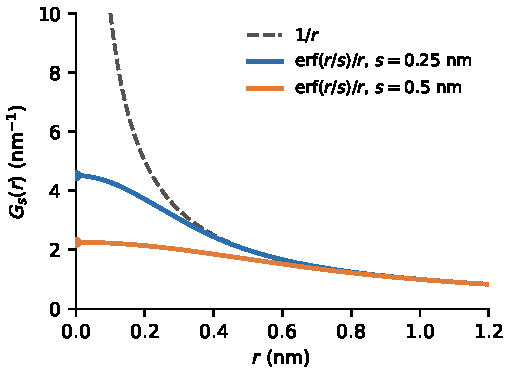
\includegraphics[width=0.5\textwidth]{fig/kernel.pdf}
  \caption{The smoothed Coulomb kernel $G_s(r) = \mathrm{erf}(r/s)/r$ against $1/r$; the dots are $G_s(0)$. The model's
  $s_e = 0.25$\,nm is the blue curve.}
  \label{fig:kernel}
\end{figure}

There are two reasons to smooth.
On a grid of spacing $\Delta x$ a cell is a blob of width $\sim\Delta x$; treating it as a Gaussian with $s=2\Delta x$
makes the grid sums smooth approximations of the integrals.
And physically, a classical Boltzmann gas collapses into a point ion ($e^{\kc q/rT}$ is not integrable at $r\to0$):
the electron's quantum size, 0.1--0.2\,nm at 10--50\,eV, blurs the singular well, and the bound part of the well is
the ion's.
The model uses
\begin{equation}
  s = \max\!\big(2\Delta x,\ s_e\big),\qquad s_e = \opt{sfmd-pb-smoothing} = 0.25\ \mathrm{nm},
\end{equation}
everywhere the kernel appears: the ion and electron potentials, the escape depth, distant ions and the long-range ion
force.
Once the grid resolves $s_e$ ($\Delta x\le s_e/2$), refining it no longer changes the physics.
The charge, the escape and the ion directions do not depend on $s_e$; the ion kinetic energy does
(Appendix~\ref{app:validation}).

\section{The temperature}
\label{sec:temperature}

The temperature is that of an ideal gas, $T = \frac23K/N$, with $K$ the electrons' kinetic energy --- the usual
equipartition definition, since the potential energy is explicit.
$K$ is not tracked directly: the model conserves the electrons' \emph{total} energy $E_{\mathrm{tot}} = K + U$, with
the electrostatic energy $U(\vect n) = \int n\,[-\Phi + \frac12K*n]$ (electrons with ions, and half their mutual
repulsion; the ion--ion energy is GROMACS's).
Since the density depends on $T$, $T$ and $\vect n$ are found together, from
\begin{equation}
  g(T) = E_{\mathrm{tot}} - U(\vect n_T) - \tfrac32NT = 0,
\end{equation}
where $\vect n_T$ minimizes $F$ at $T$.
A hotter cloud spreads into regions of higher potential energy, so $g$ decreases monotonically and has one root,
found by a safeguarded secant iteration (Appendix~\ref{app:numerics}).

\paragraph{Temperature floor.}
A cloud can cool below any sensible temperature late in a weak explosion (in \code{gromacs-mc}, 1B7U at 8\,keV and
$10^7$ photons, $K$ reached zero with 6000 electrons still trapped; here, lysozyme at $10^{15}$\,W/cm$^2$ cools to
1.4\,eV by 200\,fs).
The solve, the evaporation and three-body recombination therefore use $\max(T, T_{\min})$, with $T_{\min}$ =
\opt{sfmd-te-min} (1\,eV with the cloud): the density never collapses into a zero-temperature well, and recombination, which grows as
$n_e^2/T$ (Section~\ref{sec:recombination}), stays finite.
The actual $T = \frac23K/N$ keeps its own bookkeeping and may go below $T_{\min}$, or below zero when
$E_{\mathrm{tot}}$ is less than the potential energy of the floored density; the floor adds no energy.
Electron-impact ionization uses the actual $T$; it vanishes at small $T$ by itself ($e^{-\Delta E/T}$).
\file{screening\_log.txt} has both temperatures, and \code{mdrun} reports how long $T$ was below the floor.
With \opt{sfmd-te-min = 0} (and in a \file{.tpr} older than version 182) the old model applies: the solve is floored
at 1\,eV, evaporation and recombination use the actual $T$, and when $E_{\mathrm{tot}} - U$ falls below zero, $K$ is
set to zero and $E_{\mathrm{tot}}$ raised to match (energy created, logged as \code{E\_clamped} in \file{pb\_log.txt}).
On lysozyme at $10^{15}$--$10^{16}$\,W/cm$^2$ up to 200\,fs the floor acts for only $\sim$0.02\,fs, when the cloud
forms, and changes nothing in the explosion; it removes the clamp (up to 3.5\,eV at $10^{16}$, 0.8\,keV with
\opt{sfmd-laser-barrier = 2}).

\section{Energy bookkeeping}
\label{sec:energy}

Tracking $E_{\mathrm{tot}}$ instead of $K$ means that the adiabatic cooling of an expanding cloud, and the heating
when an ion's charge grows under it, appear by themselves in $K = E_{\mathrm{tot}} - U$.
$E_{\mathrm{tot}}$ changes only by explicit exchanges.
Write $V_e = K*n$ for the electrons' repulsion from the last solve, scaled by $\varsigma = N/N_{\mathrm{solve}}$ for
electrons added or lost since, and
\begin{equation}
  D_k = \kc\sum_{b\ne k} q_b\,G_s(|\vect x_k-\vect x_b|) - \varsigma\,V_e(\vect x_k)
  \label{eq:Dk}
\end{equation}
for the depth of the well at atom $k$: the binding energy of an electron at rest there.
\begin{enumerate}
  \item \textbf{Work on the ions.} The cloud's force on the ions does work $W$ per step, taken from the electrons:
    $\Delta E_{\mathrm{tot}} = -\sum_a\vect F_a\cdot\vect v_a\Delta t$.
  \item \textbf{A trapped ADK electron} at atom $k$ is born at rest: $\Delta E_{\mathrm{tot}} = -D_k$.
  \item \textbf{Electron-impact ionization} at $k$ with ionization energy $P$: a cloud electron pays it, and
    the freed electron starts at rest at $k$: $\Delta E_{\mathrm{tot}} = -P - D_k$.
    \textbf{Three-body recombination} is the reverse: $\Delta E_{\mathrm{tot}} = +P + D_k$ (Chapter~\ref{ch:coll}).
  \item \textbf{A change of an ion's charge} by $\Delta q$ changes its interaction with the cloud; the kinetic energy does
    not change at that instant: $\Delta E_{\mathrm{tot}} = -\Delta q\,\varsigma V_e(\vect x_k)$.
    Unlike \code{gromacs-mc}, which books a step's charge changes at its end, each change is booked as it happens,
    before its electron: ADK fires hundreds of events in a step at onset (634 in the first step of the lysozyme test),
    and booking them together counted every new ion--electron pair of the step twice.
  \item \textbf{Evaporation} of $\delta N$ electrons with kinetic energy $\delta E$ from mean depth $\bar D$:
    $\Delta E_{\mathrm{tot}} = -(\delta E - \delta N\bar D)$; with the laser barrier the depth is measured below the
    lowered escape level (Chapter~\ref{ch:laser}).
  \item \textbf{The laser}: heating adds its absorbed energy to $K$ and $E_{\mathrm{tot}}$; a spill removes the spilled
    electrons' kinetic energy ($\frac32T$ each) and their electrostatic energy (Chapter~\ref{ch:laser}).
  \item \textbf{A grid rebuild} changes $U$ for numerical reasons only; the change is moved into $E_{\mathrm{tot}}$ so
    that $K$ does not jump.
\end{enumerate}
An electron that escapes at birth never joins the cloud; it only raises the net charge.
\file{energy\_ledger.txt} and \file{pb\_log.txt} record these terms (Chapter~\ref{ch:output}).

\section{Forces on the ions}

An ion of charge $q_a$ has potential energy $-q_a\varsigma V_e(\vect x_a)$ in the cloud, so the cloud pulls on it with
\begin{equation}
  \vect F_a = q_a\,\varsigma\,\nabla V_e(\vect x_a),
\end{equation}
from central differences on the grid, interpolated to the atom (outside the grid: a point charge at the cloud's
centroid).
The forces are added to the GROMACS forces every step on every rank, and their work is booked (item~1).
Between solves the ions move through the fixed electron potential.

\section{Escape or trapping}
\label{sec:escape}

An ADK electron is born at rest at its atom $k$.
It escapes if the depth~\eqref{eq:Dk} at its atom, of the same smoothed ion potential and the same cloud the solve
uses, is at or below the escape level, $D_k\le\Delta W$, and is trapped otherwise.
$\Delta W$ is the laser's lowering of the escape level (Section~\ref{sec:barrier}); without the barrier it is 0, and
the first electron of a neutral sample ($D=0$) leaves.
(\code{gromacs-mc} tests $\varepsilon > D_k$ strictly; with $\varepsilon = 0$ for every ADK electron that would trap
the first one.)
The atom's own new charge is left out: the electron leaves before the atom's remaining electrons rearrange.
An escaped electron adds one to the net charge $Q$; a trapped one adds one to $N$ and is booked as item~2.
Each electron is tested once, at birth: an escaped one cannot be recaptured, and a trapped one leaves only by
evaporation.

\section{Evaporation}
\label{sec:evaporation}

A well of finite depth cannot hold the tail of a Maxwell distribution: an electron whose kinetic energy exceeds its
local depth $D(\vect x) = -V(\vect x)$ is unbound and leaves, and collisions keep refilling the tail.
This evaporation (\opt{sfmd-evaporation = 1}, the default) matters late in the explosion, when the well is shallow and
the cloud still hot.
For a Maxwell distribution at $T$, the fraction of electrons above $D$ and the fraction of their kinetic energy above
$D$ are regularized incomplete gamma functions of $x = D/T$~\cite{abramowitz1964}:
\begin{equation}
  Q(\tfrac32,x) = \mathrm{erfc}\sqrt x + 2\sqrt{x/\pi}\,e^{-x},\qquad
  Q(\tfrac52,x) = Q(\tfrac32,x) + \tfrac{4}{3\sqrt\pi}x^{3/2}e^{-x}.
\end{equation}
The energy tail is the larger (Fig.~\ref{fig:tails}), so evaporation cools the cloud.
Summed over the cells of the last solve (binned by depth into 4000 bins once per solve),
$\delta N^{\mathrm{tail}} = \sum_i n_iQ(\frac32,x_i)$ and $\delta E^{\mathrm{tail}} = \frac32T\sum_in_iQ(\frac52,x_i)$.
The tail refills at the electron--electron collision rate~\cite{nrl}
\begin{equation}
  \nu_{ee} = 2.91\times10^{-6}\,n_e[\mathrm{cm^{-3}}]\,\ln\Lambda\,T^{-3/2}\ \mathrm{s^{-1}},\qquad
  \ln\Lambda = \max\big(2,\ 24-\ln(\sqrt{n_e}/T)\big),
\end{equation}
at the mean density $n_e = N/(\frac43\pi R^3)$, and every MD step a fraction $\phi = \min(1,\nu_{ee}\Delta t)$ of it
leaves: $N$ and $K$ fall by $\phi\varsigma\,\delta N^{\mathrm{tail}}$ and $\phi\varsigma\,\delta E^{\mathrm{tail}}$, the
net charge $Q$ rises, and the leavers' total energy is booked (item~5).
How many electrons evaporate depends on the box (Appendix~\ref{app:numerics}); the total that escapes, at birth and by
evaporation, does not.

\begin{figure}[t]
  \centering
  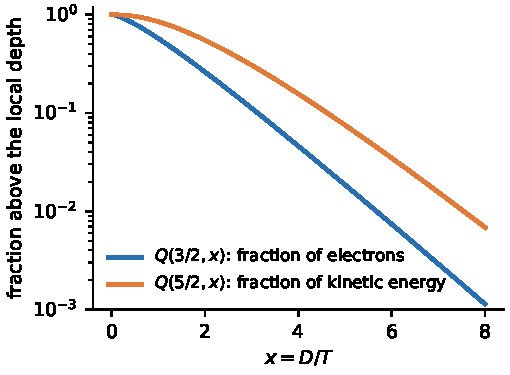
\includegraphics[width=0.5\textwidth]{fig/tails.pdf}
  \caption{The Maxwell tails above a depth $D$: the fraction of electrons $Q(\frac32,D/T)$ and of their kinetic energy
  $Q(\frac52,D/T)$.}
  \label{fig:tails}
\end{figure}

\section{Assumptions}

\begin{itemize}
  \item One temperature, instantaneous equilibrium: hot spots are averaged out at the next solve.
  \item Classical mean field: no degeneracy, exchange or correlation below the scale $s_e$; $s_e$ has a physical size
    but is not derived from first principles.
  \item Electrons frozen between solves (0.2\,fs), adequate while the ions move much less than a grid cell in that
    time.
  \item Escape at birth, by evaporation and by the laser's spill only; evaporation at the mean electron--electron
    collision rate, an estimate rather than a kinetic calculation.
  \item Electrons born at rest: no drift or rescattering energy from the field.
  \item Far from the sample the cloud is a point charge.
\end{itemize}

\chapter{The laser on the cloud}
\label{ch:laser}

\devnote{This chapter describes the \code{pb-electrons} branch. The barrier and the heating are on by default with the
cloud (\opt{sfmd-laser-barrier = 1}, \opt{sfmd-laser-heating = 1}).}

The trapped electrons sit in the field of the pulse as much as the atoms do.
Two effects are modelled, both from the cycle-averaged picture of a cluster in a strong
field~\cite{ditmire1996,saalmann2006,fennel2010}: the field lowers the barrier the electrons must cross to leave, and it
heats them.
Without these the cloud is far too stable: a field-free cloud keeps $\sim$98\,\% of the electrons at every intensity,
including $10^{17}$\,W/cm$^2$, where in reality the sample is stripped (Appendix~\ref{app:validation}).

\section{The barrier}
\label{sec:barrier}

A sample of net charge $Q$ (the electrons that have left) in a uniform field $E_0$ has a potential
$-\kc Qe/r - eE_0 z$ along the field: the Coulomb well tilts and a saddle opens on the downhill side at
\begin{equation}
  r_s = \sqrt{\kc Q/E_0},\qquad \Delta W = 2\sqrt{\kc Q\,e\,E_0}
\end{equation}
below the field-free escape level (zero at infinity), with $\kc = 1.44$\,eV\,nm.
An electron less bound than $\Delta W$ can leave over the saddle.
With \opt{sfmd-laser-barrier = 1} the model uses this lowering, with the envelope amplitude $E_0(t)$ of the current
step, in three places:
\begin{description}
  \item[Escape at birth:] a new electron escapes if the depth at its atom is $D_k\le\Delta W$ (Section~\ref{sec:escape}).
  \item[The spill:] after every solve, the cloud cells whose depth $-V$ is below $\Delta W$ are emptied at once.
    Their electrons leave with their kinetic energy, $\frac32T$ each, and their electrostatic energy, computed exactly
    as $U$ before minus $U$ after; the rest of the cloud keeps its kinetic energy.
    $Q$ grows by the spilled number, so $\Delta W$ grows (as $\sqrt Q$) and the well deepens (as $Q$): the cloud is
    solved again and spills again, up to 6 rounds, until less than 1\,\% of it (or fewer than 2 electrons) would
    spill.
  \item[Evaporation:] the depth of each cell in the Maxwell-tail evaporation (Section~\ref{sec:evaporation}) is
    measured below the lowered level, $-V-\Delta W$; the leavers still take their true potential energy out of the
    cloud.
\end{description}
The cloud itself is overdense ($\omega_p$ several times $\omega$), so the laser does not reach inside it and the
equilibrium solve is unchanged; only the level the electrons must stay below moves.
The picture holds while the saddle lies outside the sample ($r_s>R$); when it does not, $\Delta W$ exceeds the well and
the cloud spills entirely, which is also what happens.
\file{laser\_log.txt} has $E_0$, $Q$, $N$, $\Delta W$, $r_s$ and the spill, escape and evaporation counts at every solve.

\paragraph{The instantaneous field.}
With \opt{sfmd-laser-barrier = 2} the spill and the evaporation level follow the instantaneous field,
$2\sqrt{\kc Q e|E(t)|}$, which breathes twice per optical cycle (2.8\,fs at 850\,nm); the solves, about 14 per cycle at
0.2\,fs, resolve it.
The escape at birth keeps $E_0$, since ADK electrons are born near the field crests.
On lysozyme mode 2 gave the same charges, ion energies (within 2\,\%) and directions as mode 1, with more spill and
less evaporation about 1\,fs earlier, but more seed noise and clamped cloud energy in 3 of 24 runs (the jumping level
lets a cold cloud's tail evaporate in bulk between solves).
Mode 1 is recommended; mode 2 is a check.

\section{Heating}
\label{sec:heating}

The cloud absorbs energy from the laser by inverse bremsstrahlung: electrons driven by the field collide with the ions
and turn the quiver motion into heat.
For a sample much smaller than the wavelength the cycle-averaged absorption is that of a small dielectric particle with
the Drude permittivity~\cite{ditmire1996},
\begin{equation}
  \varepsilon = 1 - \frac{\omega_p^2}{\omega(\omega+i\nu)},\qquad
  P = \frac{\omega}{2}\,\varepsilon_0\,\mathrm{Im}\,\varepsilon\;|E_{\mathrm{in}}|^2\,V,
\end{equation}
with the plasma frequency $\omega_p$ of the cloud's mean density $n_e = N/V$, $V = \frac43\pi R^3$, and the field inside
the cloud $E_{\mathrm{in}}$.
$P\Delta t$ is added to the cloud's kinetic and total energy every MD step (work from outside, \code{laser heating} in
the run summary and \file{laser\_log.txt}).

\paragraph{The field inside.}
For a sphere (\opt{sfmd-heating-shape = sphere}) $E_{\mathrm{in}} = 3E_0/(\varepsilon+2)$.
The formula covers the three regimes of a cluster: shielding while the cloud is dense ($\omega_p\gg\omega$, small
$E_{\mathrm{in}}$), the Mie resonance as it expands through $\omega_p = \sqrt3\,\omega$ (a density of $3n_c$,
$n_c\approx1.55\times10^{21}$\,cm$^{-3}$ at 850\,nm), and the resistive regime $\nu\gg\omega$.
With \opt{sfmd-heating-shape = ellipsoid} (the default) the cloud has the shape of the sample's gyration ellipsoid,
semi-axes $a_i$, and the field along each axis is $E_{0,i}/(1+L_i(\varepsilon-1))$, with the depolarization factors
\begin{equation}
  L_i = \frac{a_1a_2a_3}{2}\int_0^\infty\frac{\dd s}{(s+a_i^2)\sqrt{(s+a_1^2)(s+a_2^2)(s+a_3^2)}}
      = \frac{a_1a_2a_3}{3}\,R_D(a_j^2,a_k^2,a_i^2)
\end{equation}
(Carlson's elliptic integral; $\sum L_i = 1$, $L_i = \frac13$ for a sphere).
The model has no field direction, so it averages over the orientation of the polarization:
\begin{equation}
  |E_{\mathrm{in}}|^2 = \frac{E_0^2}{3}\sum_i\big|1+L_i(\varepsilon-1)\big|^{-2}.
\end{equation}
The resonance then falls at $n_c/L_i$ for each axis rather than at $3n_c$; lysozyme starts at $L$ = 0.21, 0.37, 0.41.
On lysozyme the ellipsoid gave 13\,\% more heating and 6\,\% more ion energy at $10^{15}$\,W/cm$^2$ and about 1\,\% at
$10^{16}$, directions within the noise.

\paragraph{The collision rate.}
$\nu$ is the electron--ion collision rate~\cite{nrl},
\begin{equation}
  \nu_{ei} = 2.91\times10^{-6}\,Z\,n_e[\mathrm{cm^{-3}}]\,\ln\Lambda\,T^{-3/2}\ \mathrm{s^{-1}},\qquad
  Z = \frac{\sum q_a^2}{\sum q_a},\qquad \ln\Lambda = \max\big(2,\ 24-\ln(\sqrt{n_e}/T)\big),
\end{equation}
at the cloud's temperature (at least the floor, Section~\ref{sec:temperature}), with two corrections:
\begin{description}
  \item[The cap] $\nu_{ei}\le$ \opt{sfmd-heating-nu-cap}$\cdot\omega_p$ (1): a cold, dense cloud is strongly coupled, and
    the weak-coupling formula would give $\nu\gg\omega_p$; a collision rate saturates near the plasma frequency.
    The cap is an order-of-magnitude choice, not fitted.
    It matters only while the cloud is cold and dense: on lysozyme at $10^{15}$\,W/cm$^2$, a cap of 0.5 gave 16\,\% less
    heating and 8\,\% less ion energy; at $10^{16}$ nothing.
    No cap gave the same as cap 1.
    0 removes it.
  \item[Surface damping] $\nu \mathrel{+}= A\,\bar v/R$ with $\bar v = \sqrt{8T/\pi m_e}$ and $A$ =
    \opt{sfmd-heating-surface} (1): the electrons of a nm-sized cloud cross it in $R/\bar v$, which damps its plasmon
    (Kreibig damping~\cite{kreibig1995}).
    Without it only $\nu_{ei}$ damps the resonance, and a hot, thin cloud ($\nu/\omega\sim10^{-5}$) can absorb MeV
    within a step when a solve lands on the resonance: 15--19\,MeV heating outliers in about 1 of 8 runs at
    $10^{16}$--$10^{17}$\,W/cm$^2$.
    With $A=1$ ($\nu_s/\omega\approx$ 0.5--0.9 near the resonance) the outliers are gone and the seed spread of the ion
    energy falls from $\pm90$ to $\pm28$\,keV at $10^{16}$.
    $A$ is of order 1 in the literature and not fitted; from $A$ = 0.5 to 2 the ion energy at $10^{16}$ rises by 2.3\,\%,
    directions unchanged.
\end{description}

\section{Linear polarization}
\label{sec:polarization}

\devnote{\opt{sfmd-laser-polarization} is new (tpr 185) and not validated beyond the checks below. Default 0: the laser
without a direction, as in the rest of this chapter.}

The barrier above is lowered all round, which overstates escape: the real saddle exists only on the downhill side of
the field, on the polarization axis, and moves from one pole to the other every half cycle.
With \opt{sfmd-laser-polarization = x}, \code{y} or \code{z} the field $E(t)\,\hat e$ of the pulse (carrier included)
acts on the cloud and the ions directly:
\begin{description}
  \item[In the solve.] The laser's potential energy of an electron, $U_L = eE(t)\,(\mathbf r-\mathbf c)\cdot\hat e$
    ($\mathbf c$ the heavy-atom centre), is added to the potential of the PB solve, $V = -\Phi + Kn + U_L$, so the cloud
    polarizes: it shifts along $\hat s = -\mathrm{sign}(E)\,\hat e$, the direction the field pushes electrons.
    The cloud's plasma frequency is several times the laser's, so it follows the field adiabatically; the solves sample
    the carrier (14 per cycle at 0.2\,fs and 850\,nm; \code{grompp} warns below 8) and the field is held in between.
  \item[The escape level] is the saddle on the downhill side. Along $\hat s$, outside the sample,
    \begin{equation}
      U(r) = -\frac{\kc Q}{r} - \frac{\kc P}{r^2} - |E|\,r,\qquad P = \mathbf p\cdot\hat s,
    \end{equation}
    with $\mathbf p$ the dipole of ions and cloud about $\mathbf c$ from the last solve (the shifted cloud gives $P<0$,
    which raises the saddle). The saddle $r_s$ is the largest root of $|E|r^3-\kc Qr-2\kc P=0$, the level
    $U_s = U(r_s)$; for $P=0$ it is the barrier of Section~\ref{sec:barrier}, $U_s=-\Delta W$.
    If that root lies inside the sample ($r_s<R_e$, the gyration ellipsoid's radius along the axis), or there is
    none because the dipole term wins (a strongly polarized cloud of small $Q$), $U$ falls all the way out beyond
    $R_e$ and the level is $U(R_e)$, the highest point on the way out. (The first version took the root, or for no
    root a point deep inside the sample, where the dipole term made the level huge; a neutral cloud along the long
    axis was then held at $10^{17}$\,W/cm$^2$ and absorbed 130\,MeV in one of 8 runs.) Beyond the saddle plane
    the field term is held at its value there: those cells are outside the trap.
  \item[Escape] is then decided by energy against $U_s$: a cell spills if $V\ge U_s$, a newborn electron escapes if
    $-D_k + U_L(\mathbf x_k)\ge U_s$, and evaporation measures each cell's depth as $U_s - V$. Electrons on the
    up-field side are lifted by $U_L$, those on the down-field side lowered; the cloud's tail beyond the saddle region
    goes first. Both \opt{sfmd-laser-barrier} modes behave the same with the polarization (it needs one of them on).
  \item[The ions] feel $qE\,\hat e$ of the solve's field, so that ions and cloud together feel the net charge's
    $QeE$.
  \item[Heating] with the ellipsoid uses the field along the axis, $|E_{\mathrm{in}}|^2 = E_0^2\sum_i (\hat e\cdot\hat u_i)^2
    |1+L_i(\varepsilon-1)|^{-2}$ with the sample's principal axes $\hat u_i$, instead of the orientation average.
\end{description}

\paragraph{Energy.}
The cloud's energy ledger is kept without the field term ($E_{\mathrm{kin}} = E_{\mathrm{tot}} - U$, $U$ the
electrostatic energy of cloud and ions), and the field's work on the cloud between two solves,
$\int E\,\dd X$ with $X = \sum_i n_i\,\mathbf r_i\cdot\hat e$, is added to $E_{\mathrm{tot}}$ with the mean of the two
solves' fields. For a cloud that follows the field linearly this sum telescopes to zero over a cycle; with the new
field alone it would put $\frac12\alpha\,\Delta E^2$ into the cloud at every solve, several keV per solve for lysozyme at
$10^{16}$\,W/cm$^2$. Births, captures, evaporation and spills update $X$ with the electrons' positions, so the work
done on an electron born at its atom as it joins the shifted cloud is counted. The run's end reports the cumulative
polarization work. The part stored in the shifted cloud, $\frac12\alpha E^2$, returns as the field falls; electrons born at
their atoms into the shifted cloud gain about $|E|d$ each ($d$ the shift), and the down-field tail that spills was
pulled there by the field, so a cloud that changes during the pulse keeps a net gain (643\,keV for lysozyme at
$10^{16}$\,W/cm$^2$, against 1.6\,MeV of heating); \file{laser\_log.txt} gets the solve's field,
$p_{\hat e}$, the work and the solves without a saddle as extra columns ($\Delta W$ and $r_s$ there are $-U_s$ and
the saddle's distance).

\section{What is left out}

\begin{itemize}
  \item The field's direction, unless \opt{sfmd-laser-polarization} is set: the barrier is lowered all round, not
    only along the polarization, and the heating is orientation-averaged.
  \item Quiver motion and the electrons' response within a cycle (except the spill with mode 2).
  \item Heating at the surface (vacuum or Brunel heating), and the density profile: one mean density.
  \item The energy of electrons that leave: they take their thermal energy, not a drift energy from the field.
\end{itemize}

\chapter{Collisions in the cloud}
\label{ch:coll}

\devnote{This chapter describes the \code{pb-electrons} branch. Impact ionization is on by default with the cloud
(\opt{sfmd-collisions = 1}); recombination is off (\opt{sfmd-coll-recombination = 0}).}

The trapped electrons are hot and dense, and they collide with the ions: they ionize further, and once the pulse is
over and the cloud cools they can be captured again.
Both are \code{gromacs-mc}'s built-in Lotz channels (\opt{mcmd-coll-data = lotz}), restricted to the valence shell that
ADK ionizes.

\section{Electron-impact ionization}

An ion in charge state $q$ at atom $k$ is ionized by the cloud at the rate $n_e(\vect x_k)\langle\sigma v\rangle$, with
$n_e(\vect x_k)$ the cloud density at the atom (from the last solve, scaled to the current $N$) and Lotz's Maxwellian
rate coefficient~\cite{lotz1968}
\begin{equation}
  \langle\sigma v\rangle = 6.7\times10^{-7}\,a\,\xi\,T^{-3/2}\,\frac{E_1(P/T)}{P/T}\ \ \mathrm{cm^3\,s^{-1}},\qquad a = 4.5,
\end{equation}
$\xi$ the number of electrons left in the valence shell (H 1, C 4, N 5, O 6, S 6, minus $q$), $P$ the ionization
energy of the state (Table~\ref{tab:adk}), $T$ the cloud's actual temperature in eV and $E_1$ the exponential integral.
The new electron stays in the cloud, at rest at the atom; a cloud electron pays $P$
(Section~\ref{sec:energy}, item~3).
An event the cloud cannot pay ($K<P$) is not made.
Impact ionization is tried every step for every atom that ADK left alone, while the cloud has at least one electron.

On lysozyme at $10^{15}$\,W/cm$^2$ impact ionization raises the ion charge by a third (1.29 to 1.72 per atom) but the new
electrons stay trapped: the net charge, the ion energy (+6\,\%) and the directions hardly change.
At $10^{16}$ it adds 2.5\,\% to the charge, at $10^{17}$ nothing.

\section{Three-body recombination}
\label{sec:recombination}

Recombination is the inverse of impact ionization, from detailed balance (Saha):
\begin{equation}
  \alpha_3 = n_e^2\,\langle\sigma v\rangle_{q-1\to q}\,e^{P/T}\,\frac{g_{q-1}}{g_q}\,\lambda^3,\qquad
  \lambda^3 = 1.656\times10^{-22}\,T^{-3/2}\ \mathrm{cm^3},
\end{equation}
with the rate coefficient of the lower state, its ionization energy $P$, and the statistical weights of the valence
shell, $g = \binom{n_{\mathrm{shell}}}{\xi}$ ($n_{\mathrm{shell}}$ = 2 for H, 8 for C, N and O, 18 for S, its M shell).
The captured electron leaves the cloud from rest at the atom, and its binding energy $P$ goes to the cloud
(Section~\ref{sec:energy}, item~3).
Ionization and recombination are drawn together: one random number decides whether an event happens, with the total rate,
and which one.

The rate grows as $n_e^2T^{-3}$, so it uses the floored temperature $\max(T,T_{\min})$ (Section~\ref{sec:temperature}),
which caps it where the cloud cools towards zero; ionization uses the actual $T$, where it vanishes by itself.

\paragraph{When.}
\opt{sfmd-coll-recombination = 2} recombines only after the pulse: past the peak and below 1\,\% of the peak
intensity.
\opt{= 1} recombines at all times.
During the pulse that is wrong for this model: recombination captures into the ground state, and the laser re-ionizes
the atom at once; on lysozyme this capture--ADK pump made 9 times as many ADK events and 22\,\% more ion energy.
Real three-body capture goes into highly excited states, which the field would strip again without much happening.
Mode 1 is a diagnostic upper bound.

On lysozyme at $10^{15}$\,W/cm$^2$, recombination after the pulse gives back most of the charge impact ionization added
(1.72 to 1.35 per atom) and leaves the explosion as it was --- as in \code{gromacs-mc}, where recombination cycles around
equilibrium without changing the dynamics.
It is the sensible choice when charge states matter.

\section{Limitations}

\begin{itemize}
  \item Valence shell only, the states of Table~\ref{tab:adk}: no inner-shell ionization.
  \item Ground-state capture (see above), and no excitation.
  \item At most one event per atom and step; at the densities at the atoms (up to $10^{24}$\,cm$^{-3}$) the rates can
    exceed $1/\Delta t$, which then limits them --- relevant only for the fast cycling of mode 1.
  \item The local density from the last solve, the temperature of the whole cloud.
\end{itemize}

\chapter{Output}
\label{ch:output}

The standard GROMACS output (\file{.trr}, \file{.edr}, \file{.gro}, \file{.log}, \file{.cpt}) is written as usual.
The module writes into \file{simulation\_output/} in the directory \code{mdrun} runs in.
Times in the files are GROMACS times in ps unless the header says otherwise; atom indices are 0-based.

\section{Run summaries}
\label{sec:summaries}

At the first step \code{mdrun -ionize} prints a summary to stderr and the \file{.log}:
\begin{lstlisting}
 MolDStruct SF (strong-field ionization, ADK) with the trapped-electron cloud - DEVELOPMENT BUILD
 System        1960 atoms (H 959, C 613, N 193, O 185, S 10), ionization charge +0 at the start
 Pulse         0.005 J, 850 nm, FWHM 2 fs, peak at 2 fs, focus 30000 nm
               peak intensity 3.32e+17 W/cm^2, peak field 1.58e+03 V/nm
 Run           600 steps x 2 as = 1.2 fs; seed 7 (GMX_SFMD_SEED); 4 ranks

 Processes
   ADK tunnel ionization                    on (always)
   trapped electrons (Poisson-Boltzmann)    on   sfmd-electrons = pbgrid
       grid                                 s_e 0.25 nm, 2.5 cells/s_e, box <= 3 R, <= 384 cells, solve every 0.2 fs
       evaporation                          on
       laser barrier                        on: envelope field (sfmd-laser-barrier = 1)
       laser heating                        on   Drude ellipsoid, nu_ei <= 1 omega_p, surface damping A = 0
       electron-impact ionization           on   Lotz
       three-body recombination             off
       temperature floor                    1 eV: solve, evaporation, recombination at >= it
   ion-ion forces                           all pairs

 Output        simulation_output/: event logs (sfmd-detailed-output = 1), charges_over_time.bin every 50 steps;
               autostop off

 Warnings (settings outside what was tested)
   - peak intensity 3.3e+17 W/cm^2: the cloud was tested at 1e15-1e17 W/cm^2 (lysozyme, 850 nm, 15 fs)
   - sfmd-heating-surface = 0: the Mie resonance is undamped (15-19 MeV heating outliers in ~1 of 8 runs ...)
\end{lstlisting}
With a schedule the run line gives the end time and the stages are listed.
The warnings cover what the tests found to matter: the cloud without the barrier or heating, barrier mode 2, no surface
damping, a collision-rate cap other than 1, recombination mode 1, the old temperature model, a coarser solve or other
smoothing, an intensity outside $10^{15}$--$10^{17}$\,W/cm$^2$, harmonic bonds, a step above 2\,as, all pairs above 10\,000
atoms, a cut-off without long range, and a pulse that ionizes nothing.

At the end:
\begin{lstlisting}
 MolDStruct SF: end of the run at 1.2 fs (nsteps)
 Charge        total +5546, 2.830 per atom; per element: H 1.00 C 4.00 N 5.00 O 6.00 S 6.00
 Events        ADK 5525, electron impact 21, three-body recombination 0
\end{lstlisting}
followed by the cloud's lines: electrons escaped at birth, trapped, evaporated and spilled, the laser heating, the final
$N$, $Q$ and $T$, the solves, the energy ledger with \code{E\_clamped}, the impact ionizations and recombinations with the
energy they moved, and how long $T$ was below the floor.
The ADK count is the final minus the initial charge, less impact ionizations, plus recombinations: exact with any number
of ranks, with or without the event logs.
A run stopped by the autostop says so (\code{autostop 2: ion directions settled, 60.0 fs after the pulse peak}).

\section{Files}

\begin{longtable}{@{}p{0.27\textwidth}p{0.68\textwidth}@{}}
\toprule
file & content \\
\midrule
\endhead
\multicolumn{2}{@{}l}{\emph{Always (with -ionize)}}\\
\file{charges.txt} & at the end: atom (1-based) and charge; read back by \opt{sfmd-initial-charges = 1} \\
\file{masses.bin} & float32 masses, once (the element of each atom) \\
\multicolumn{2}{@{}l}{\emph{With \opt{sfmd-detailed-output = 1}}}\\
\file{pulse\_profile.txt} & every step: $t$, $I(t)$ [W/cm$^2$], $E(t)$ [V/m], pulse active (0/1) \\
\file{mean\_charge\_vs\_time.txt} & every step: $t$, mean ion charge, ionizations this step, pulse active \\
\file{charges\_over\_time.bin} & float32, one frame of all atoms every \opt{sfmd-charge-output-stride} steps; frame $k$ at
  $t_{\mathrm{init}} + k\cdot$stride$\cdot\Delta t$ with the \file{.tpr}'s $\Delta t$ and stride (a schedule rescales
  the stride to keep that spacing) \\
\file{transition\_log.txt} & per ADK event: $t$, atom, element, charge before and after, field, rate, probability,
  random number \\
\file{collisional\_log.txt} & per impact ionization or recombination (after $<$ before): $t$, atom, element, charge
  before and after, $T$, $n_e$ at the atom [cm$^{-3}$], rate, probability, random number \\
\multicolumn{2}{@{}l}{\emph{With the cloud (header lines name the columns)}}\\
\file{pb\_log.txt} & per solve: $N$, $Q$, $T$, spacing, ions outside the box, Newton and CG iterations, residual,
  wall time, mean and maximum depth, work and $\Delta U$, $K$, \code{E\_clamped}, core charge, convolutions, rebuilds,
  $T$ iterations \\
\file{laser\_log.txt} & per solve: $E_0$, $Q$, $N$, $\Delta W$, $r_s$, $R$, spilled (this solve, rounds, total),
  escaped at birth and evaporated totals, $T$, heating [eV/fs] and total, $\nu/\omega$, $|E_{\mathrm{in}}|/E_0$,
  $Z_{\mathrm{eff}}$ \\
\file{screening\_log.txt} & every 100 steps (a \emph{step} column): escaped, trapped, fraction, mean energy, $R$, Debye
  length, evaporated, $T$, pressure work \\
\file{energy\_ledger.txt} & every 100 steps: step and $t$, the cumulative ion--ion and ion--cloud jumps of charge
  changes, the field work, $K$, $N$ \\
\file{pbg\_box.txt} & the adaptive box and grid at each rebuild \\
\file{pbg\_lr.txt} & with long range: per refresh, the cut-off, smoothing, ions outside, $U_{\mathrm{lr}}$, work, and
  the error against all pairs with \env{GMX\_SFMD\_PBG\_LR\_CHECK} \\
\multicolumn{2}{@{}l}{\emph{With \opt{sfmd-autostop = 2}}}\\
\file{autostop\_dirs.txt} & per check [fs]: the median heavy-ion turn, the predicted rest, the number of ions \\
\bottomrule
\end{longtable}
The ion charges are in \file{mean\_charge\_vs\_time.txt} and \file{charges.txt}; the sample's net charge is the ion charge
minus the cloud's $N$.

\section{The summary tool}

\file{tools/sfmd\_output.py} (Python~3, numpy, matplotlib for the figures; no GROMACS) reads a run's
\file{simulation\_output/}, or the run directory holding it:
\begin{lstlisting}
sfmd_output.py summary     run/              # run, final charge states, events per element and per 5 fs, cloud, autostop
sfmd_output.py charges     run/ --every 10   # mean charge per element over time
sfmd_output.py transitions run/ --type adk,impact,recomb --atom 12 --tmin 20 --tmax 40
sfmd_output.py plot        run/ [--gif [--no-h]] [--extract]
\end{lstlisting}
\code{plot} writes \file{overview.png} (Fig.~\ref{fig:overview}); \code{--gif} an explosion movie in three views along
the sample's principal axes, coloured by charge; \code{--extract} text copies of the events and the charge frames.
In Python, \code{import sfmd\_output as so} gives \code{so.read\_events}, \code{so.read\_charges} (frame times and
charges), \code{so.elements} and \code{so.table}.

Every file goes on a time axis from what the run wrote, never as steps $\times\,\Delta t$, which is wrong under a
schedule: \file{screening\_log.txt} is timed by interpolation in \file{energy\_ledger.txt}, which has both step and time,
and the charge frames by the \file{.tpr}'s $\Delta t$ and stride read from the \file{.log}.

\begin{figure}[t]
  \centering
  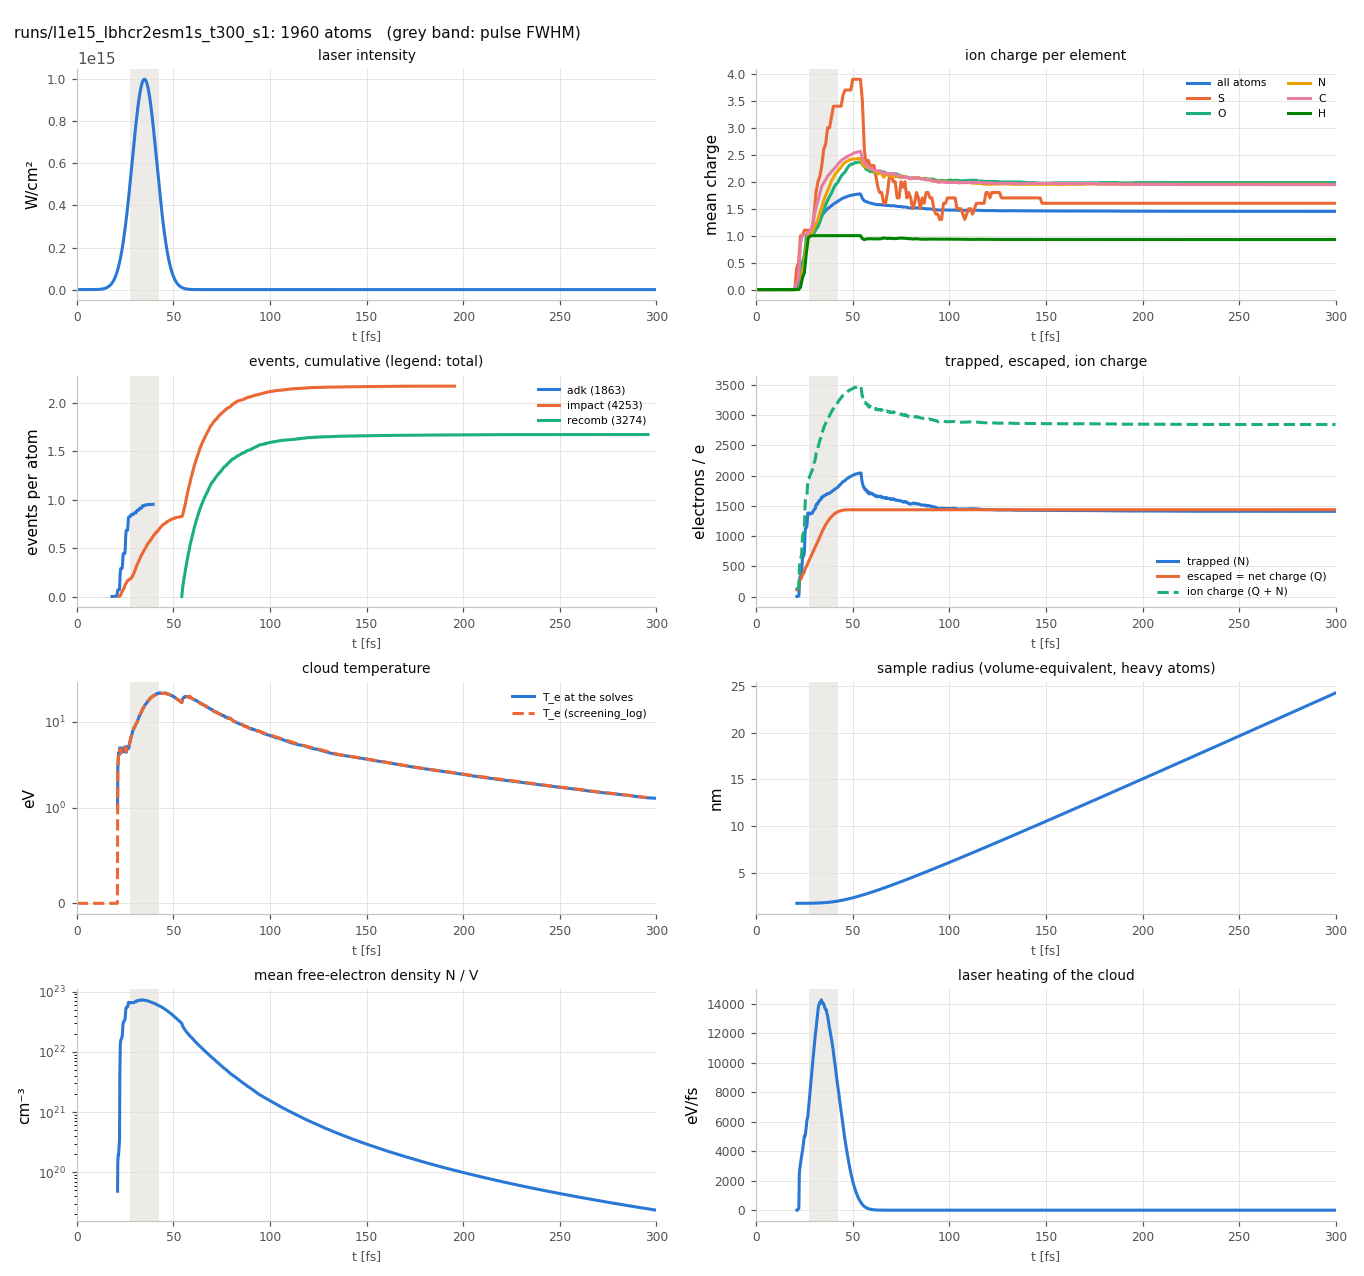
\includegraphics[width=\textwidth]{fig/overview.png}
  \caption{\code{sfmd\_output.py plot} of a lysozyme run at $10^{15}$\,W/cm$^2$ with the recommended cloud and
  recombination after the pulse, under the schedule \code{65:0.01:0.2 95:0.1:2 135:0.1:5}. The grey band is the pulse
  FWHM. The temperature from \file{screening\_log.txt} (dashed), timed through the ledger, lies on the solves' through
  the three changes of step.}
  \label{fig:overview}
\end{figure}

\chapter{mdp options}
\label{ch:mdp}

Every \opt{sfmd-*} option is inert without \code{mdrun -ionize}: without it the run is stock GROMACS 4.5.4 whatever
the \file{.mdp} says.
\code{grompp} refuses an unknown \opt{sfmd-*} key (a typo), a key given twice, the old \code{userint}/\code{userreal}
slots and the two renamed options, naming the replacement each time (Appendix~\ref{app:misc}).
The last column is the \file{.tpr} version that introduced the option; an older \file{.tpr} reads with the value
that keeps its behaviour.

\section{GROMACS settings}

\begin{tabularx}{\textwidth}{@{}l l X@{}}
\toprule
option & value & why \\
\midrule
\code{dt} & 0.000002 (2\,as) & the tested step; the run summary warns above it \\
\code{morse} & \code{yes} & harmonic bonds neither weaken nor break (Chapter~\ref{ch:ff}) \\
\code{pbc}, \code{coulombtype} & \code{no}, \code{Cut-off} & an isolated sample; needed by \opt{sfmd-pb-long-range = auto} \\
\code{rcoulomb}, \code{rvdw}, \code{rlist} & 0 (all pairs) & set by \code{grompp} with the cloud and \code{auto} \\
\code{integrator} & \code{md} & leap-frog; \opt{sfmd-schedule} needs it \\
\bottomrule
\end{tabularx}

\section{Pulse and run control}

\begin{longtable}{@{}p{0.33\textwidth}p{0.12\textwidth}p{0.39\textwidth}l@{}}
\toprule
option & default & meaning & tpr \\
\midrule
\endhead
\opt{sfmd-pulse-peak-time} & 0 & centre of the Gaussian pulse [fs] & 75 \\
\opt{sfmd-pulse-fwhm} & 0 & full width at half maximum of the intensity [fs] & 75 \\
\opt{sfmd-pulse-energy} & 0 & pulse energy [J] & 75 \\
\opt{sfmd-pulse-focal-diameter} & 0 & diameter of the (uniform) focal spot [nm] & 75 \\
\opt{sfmd-pulse-wavelength} & 0 & wavelength [nm] & 75 \\
\opt{sfmd-autostop} & 0 & 1: stop once $E_{\mathrm{kin}}/E_{\mathrm{tot}}$ exceeds \opt{sfmd-autostop-energy-ratio}
  (after step 10\,000); 2: once the ion directions have settled & 75/183 \\
\opt{sfmd-autostop-energy-ratio} & 0.99 & the ratio of autostop 1 & 75 \\
\opt{sfmd-autostop-angle} & 2 & autostop 2: predicted remaining median heavy-ion turn [deg] & 183 \\
\opt{sfmd-autostop-interval} & 5 & autostop 2: fs between checks & 183 \\
\opt{sfmd-autostop-min-time} & 60 & autostop 2: no stop before this many fs after the pulse peak & 183 \\
\opt{sfmd-schedule} & (empty) & \code{t:dt:pb ...} [fs]: from time $t$ the MD step \code{dt} and the cloud-solve
  interval \code{pb}; at most 16 stages; the first change not before the peak + $3\sigma$ & 184 \\
\opt{sfmd-initial-charges} & 0 & 1: start from \file{charges.txt}; not with the cloud & 75 \\
\opt{sfmd-detailed-output} & 0 & 1: the per-step and event files (Chapter~\ref{ch:output}) & 75 \\
\opt{sfmd-charge-output-stride} & 50 & steps between frames of \file{charges\_over\_time.bin} & 75 \\
\bottomrule
\end{longtable}

\section{The trapped-electron cloud}

\devnote{The cloud options are on the \code{pb-electrons} branch. With \opt{sfmd-electrons = pbgrid} the physics
options default to the recommended model (Chapter~\ref{ch:start}); without the cloud they are off, and setting the
barrier, heating or collisions explicitly is refused.}

\begin{longtable}{@{}p{0.33\textwidth}p{0.12\textwidth}p{0.39\textwidth}l@{}}
\toprule
option & default & meaning & tpr \\
\midrule
\endhead
\opt{sfmd-electrons} & \code{none} & \code{none}: every electron leaves; \code{pbgrid}: the Poisson--Boltzmann cloud & 175 \\
\opt{sfmd-pb-interval} & 0.2 & fs between solves & 175 \\
\opt{sfmd-pb-smoothing} & 0.25 & charge smoothing $s_e$ [nm]; the ion kinetic energy depends on it & 175 \\
\opt{sfmd-pb-cells-per-smoothing} & 2.5 & grid spacing $s_e$/this at the start & 175 \\
\opt{sfmd-pb-box-cut} & 0.02 & fraction of electrons allowed outside the adaptive box & 175 \\
\opt{sfmd-pb-box-max} & 3 & largest box half-width [$R$] & 175 \\
\opt{sfmd-pb-grid-limit} & 384 & largest grid per dimension & 175 \\
\opt{sfmd-pb-newton-tol} & 0.01 & Newton tolerance (relative) & 175 \\
\opt{sfmd-pb-long-range} & \code{auto} & 1: GROMACS does the ion pairs within \code{rcoulomb}, the grid the rest; 0: off;
  \code{auto}: all pairs up to 10\,000 atoms, above that 1 with a 2\,nm cut-off (\code{grompp} sets the cut-offs) & 175 \\
\opt{sfmd-evaporation} & 1 & the hot tail leaves over the escape level & 175 \\
\opt{sfmd-laser-barrier} & 1$^*$ & 1: the envelope field lowers the escape level; 2: spill and evaporation follow
  $|E(t)|$; 0: off & 176 \\
\opt{sfmd-laser-heating} & 1$^*$ & inverse-bremsstrahlung heating & 177 \\
\opt{sfmd-heating-nu-cap} & 1 & $\nu_{ei}\le$ this $\times\,\omega_p$; 0: no cap & 177 \\
\opt{sfmd-heating-shape} & \code{ellipsoid}$^*$ & \code{sphere} or \code{ellipsoid}: the field inside the cloud & 180 \\
\opt{sfmd-heating-surface} & 1$^*$ & surface damping $\nu_s = A\bar v/R$; 0: off & 181 \\
\opt{sfmd-collisions} & 1$^*$ & electron-impact ionization (Lotz) & 178 \\
\opt{sfmd-coll-recombination} & 0 & three-body recombination: 1 always, 2 after the pulse; needs collisions & 179 \\
\opt{sfmd-te-min} & 1$^*$ & temperature floor [eV] of the solve, evaporation and recombination; 0: the old model & 182 \\
\opt{sfmd-laser-polarization} & 0 & \code{x}, \code{y}, \code{z}: the instantaneous field along that axis in the solve,
  saddle escape level, $qE$ on the ions (development, Section~\ref{sec:polarization}); needs the barrier & 185 \\
\bottomrule
\end{longtable}
\noindent $^*$ with \opt{sfmd-electrons = pbgrid}; 0 (\code{sphere}) without the cloud.
Before 11 November 2026 these defaulted to 0 (\code{sphere}) with the cloud too.

\chapter{Environment variables}
\label{ch:env}

None of these changes the model; they are for reproducibility, tests and diagnostics.

\begin{longtable}{@{}p{0.36\textwidth}p{0.58\textwidth}@{}}
\toprule
variable & effect \\
\midrule
\endhead
\env{GMX\_SFMD\_SEED=n} & pin the ADK seed (Section~\ref{sec:seeds}); per rank, so reproducible for a given rank count \\
\env{GMX\_SFMD\_PB\_SEED="file N E"} & start from the charges in \file{file} and a seeded cloud of $N$ electrons with $E$\,eV
  kinetic energy (the comparison with \code{gromacs-mc}, \file{test/pb\_vs\_mc.sh}) \\
\env{GMX\_SFMD\_PB\_TMIN=T} & the solve's floor with \opt{sfmd-te-min = 0} (default 1\,eV) \\
\env{GMX\_SFMD\_PBG\_FFT\_THREADS=n} & threads of the solve's FFTs (default the number of ranks) \\
\env{GMX\_SFMD\_PBG\_LR\_CHECK=1} & check the long-range field against all pairs at every refresh (\file{pbg\_lr.txt}) \\
\env{GMX\_SFMD\_PBG\_OUTLAT\_CHECK=1} & check the sub-lattice sums for distant ions against the exact sum \\
\env{GMX\_SFMD\_PBG\_DENSITY=1} & write the density every 10th solve (\file{pbg\_density.bin}; large) \\
\env{GMX\_SFMD\_PB\_EDIAG=1} & energy diagnostics of the cloud \\
\env{GMX\_SFMD\_TIMING\_DETAIL=1} & section timers of the cloud (\file{pbg\_timing.txt}) \\
\bottomrule
\end{longtable}


\appendix
\chapter{Numerics of the electron model}
\label{app:numerics}

This appendix describes how the free energy of Chapter~\ref{ch:pb} is discretized and minimized, and the devices that
keep the solve affordable for $10^3$--$10^5$ atoms: an adaptive grid, an adaptive box, sub-lattices for distant ions,
and the long-range ion force from the grid.
The code is in \file{src/kernel/sfelectrons.c}; it is \code{gromacs-mc}'s, ported with mechanical renames.

\section{The grid}

The grid is a cube of $n_g^3$ nodes with spacing $\Delta x$ and half-width $h$, centred on the heavy-atom centre of
mass $\vect c$: $\vect x_{ijk} = \vect c - h(1,1,1) + \Delta x\,(i,j,k)$, $\Delta x = 2h/(n_g-1)$.
The variables are the electron counts $n_i$ at the nodes, $\sum_in_i = N$, the density $n_i/\Delta V$.
The sample radius $R = (a_1a_2a_3)^{1/3}$ is that of the heavy-atom, mass-weighted gyration ellipsoid
($a_\alpha = \sqrt{5\lambda_\alpha}$), the radius of a uniform sphere; hydrogens are left out because the fast protons
leave the cloud behind.

Each charged atom inside the grid is deposited onto its 8 surrounding nodes with cloud-in-cell (trilinear)
weights~\cite{birdsall1991,hockney1988}; the same weights interpolate grid quantities back to an atom.
With $K_{ij} = \kc G_s(|\vect x_i-\vect x_j|)$ and $\Phi_i$ the ions' potential at node $i$, the discrete free energy,
its gradient and Hessian are
\begin{gather}
  F(\vect n) = \sum_i n_i\Big[-\Phi_i + \tfrac12(\Kmat\vect n)_i + T\Big(\ln\frac{n_i}{\Delta V}-1\Big)\Big],\\
  g_i = V_i + T\ln\frac{n_i}{\Delta V},\quad V_i = -\Phi_i + (\Kmat\vect n)_i,\qquad H_{ij} = K_{ij} + \frac{T}{n_i}\delta_{ij}.
\end{gather}
At the minimum on $\sum n_i = N$ all $g_i$ are equal to $\mu$.

\section{Open-boundary convolution by FFT}

Every product $\Kmat\vect a$ is a discrete convolution, and the dominant cost.
A periodic FFT of size $n_g^3$ would add the images of neighbouring boxes; the \emph{aperiodic} convolution is computed
exactly by Hockney's method~\cite{hockney1970,eastwood1979}: embed $\vect a$ in a zero-padded grid of $(2n_g)^3$,
tabulate the kernel on the same doubled grid at the minimum-image separation, multiply the transforms and transform
back.
No two physical nodes are more than $n_g-1$ apart, so the circular convolution on the doubled grid is the aperiodic one.
The kernel transform depends only on $\Delta x$ and $s$ and is computed once per grid rebuild.
FFTW~\cite{frigo2005} in single precision, real-to-complex, multithreaded; one convolution costs two FFTs of size
$(2n_g)^3$.

\section{Newton's method}

The minimizer is found by Newton's method on the constraint surface~\cite{nocedal2006}: the step $\vect d$ minimizes
$\vect g^{\mathsf T}\vect d + \frac12\vect d^{\mathsf T}H\vect d$ subject to $\sum_id_i = 0$, i.e.
$H\vect d + \lambda\vect 1 = -\vect g$, $\vect 1^{\mathsf T}\vect d = 0$.
$H$ is symmetric positive definite, and the system ($n_g^3$ up to $10^7$ unknowns) is solved by conjugate gradients
restricted to the constraint, the projected CG of Gould, Hribar and Nocedal~\cite{gould2001}, preconditioned by the
diagonal of $H$ (Jacobi): $M_{ii} = K_0 + T/n_i$, $K_0 = 2\kc/(s\sqrt\pi)$.
The projection is built into the preconditioning step,
$\vect z = M^{-1}(\vect r - \ell\vect 1)$, $\ell = \vect 1^{\mathsf T}M^{-1}\vect r/\vect 1^{\mathsf T}M^{-1}\vect 1$,
so every search direction conserves the electron count.
CG stops at a relative projected residual of $10^{-4}$ (squared $10^{-8}$), or after 500 iterations.

The step is applied multiplicatively, $n_i\leftarrow n_i\exp(\mathrm{clip}_{[-3,3]}\,\alpha d_i/n_i)$, then renormalized
to $N$: to first order the Newton step, but every $n_i$ stays positive.
The step length $\alpha$ starts at 1 and is halved, at most 8 times, until the free energy \emph{or} the residual
falls.
(Near the target the fall of $F$, $\sim NT r_{\mathrm{PB}}^2$, is below the single-precision noise of $F$; accepting a
falling residual too avoids stalling there.)

The solve has converged when $g_i$ is the same in every occupied cell; the code measures the density-weighted spread,
\begin{equation}
  r_{\mathrm{PB}} = \frac1T\Big[\frac1N\sum_in_i(g_i-\bar g)^2\Big]^{1/2},
\end{equation}
the rms relative error of an electron's Boltzmann factor, and stops at $r_{\mathrm{PB}} <$ \opt{sfmd-pb-newton-tol}
($10^{-2}$), or after 60 Newton steps.
The first solve starts from the electrons deposited on the positive ions; later ones from the previous solution,
rescaled to the current $N$ (a warm start).
$10^{-3}$ of the electrons are spread uniformly, which keeps every $n_i>0$ and lets the cloud reach cells it had left.

\section{The temperature iteration}

$T$ and $\vect n$ are found together from $g(T) = E_{\mathrm{tot}} - U(\vect n_T) - \frac32NT = 0$
(Section~\ref{sec:temperature}):
start from the temperature of the current kinetic energy (at least \opt{sfmd-te-min}, or 1\,eV when that is 0); solve for $\vect n_T$; stop if
$|g|\le0.01\cdot\frac32NT$; otherwise move towards $T_t = (E_{\mathrm{tot}}-U)/\frac32N$ by at most a factor 4 until the
root is bracketed, then take secant steps (the geometric mean of the bracket if the secant lands within 5\,\% of an
end); at most 12 iterations, each warm-started.

\section{When the solve runs}

A solve runs every \opt{sfmd-pb-interval} (0.2\,fs, i.e.\ every 100 steps at 2\,as), and also whenever the number of
trapped electrons has grown by more than 20\,\% (plus 10) since the last one, so that the cloud keeps up during the
pulse.
In \code{gromacs-mc}, 0.2\,fs gave the 0.1\,fs results within the seed noise in ion energy, charge, escape and directions; from 0.5\,fs the
cloud stays too hot and the ion energy drops by up to 20\,\%.

\section{Adaptive grid size}

With the physical floor $s_e$ the grid only needs to resolve $s_e$.
Each rebuild chooses $n_g$ from the target spacing
\begin{equation}
  \Delta x_t = \frac{s_e}{\opt{sfmd-pb-cells-per-smoothing}}\,\max\Big(1,\frac{R}{R_0}\Big),\qquad
  n_g = 8\Big\lceil\frac{\lceil 2h/\Delta x_t\rceil+1}{8}\Big\rceil,
\end{equation}
$R_0$ the radius at the first solve, with at least 24 cells per side and at most what the sample needs at the
largest box (set at the first solve), capped at \opt{sfmd-pb-grid-limit} (384).
At the start $\Delta x = s_e/2.5 < s_e/2$, so $s=s_e$; as the sample expands every structure in the density stretches
with it, and the target spacing grows in proportion, so the grid coarsens instead of growing.
$n_g$ is a multiple of 8 to keep the FFT sizes efficient.
A sample too large for the limit gets a coarser grid late in the run, and the \file{.log} says so.

\section{Rebuilds and the adaptive box}

The grid is rebuilt at a solve when $R$ has changed by more than 10\,\% since the last rebuild, the centre has moved by
more than one cell, or the box changes.
The previous density is interpolated onto the new nodes and renormalized, the kernel transform recomputed (the FFT
plans if $n_g$ changed), and the numerical change of $U$ moved into $E_{\mathrm{tot}}$.

A box of $\pm3R$ is safe but mostly empty.
The adaptive box (\opt{sfmd-pb-box-cut}$=c$, 0.02) uses the smallest half-width that leaves at most a fraction $c$
of the electrons outside, between $1.3R$ and \opt{sfmd-pb-box-max}$\cdot R$ ($3R$); a smaller box means a finer grid
at the same cost.
The electrons outside the current box are estimated from a Boltzmann tail around the net charge $Q$ at the centre,
$n\simeq A\exp(\kc Q/(T|\vect x-\vect c|))$, with $A$ fitted to the outermost layer of cells and integrated out to the
largest box, in shells of Chebyshev distance (the box is a cube).
The box grows at once, to 5\,\% beyond the wanted size, when more than $c$ would be outside; it shrinks only to where
at most 0.1\,\% are outside (\emph{safe shrink}), so that it never cuts the cloud.
How many electrons evaporate depends on the box; the total that escapes does not.

\section{Ions outside the box}

Fast protons and some heavy ions leave the box early; their attraction still acts on the cloud.
Ions within 16 cells of the box are deposited on a correspondingly larger FFT grid.
Farther ones are added point by point, but on \emph{sub-lattices}: a distant ion's potential is smooth over the box, so
it is summed on every $S$-th node, with the largest $S = 2^L$ ($L\le4$) that satisfies $S\Delta x\le d/3$ ($d$ its
distance from the box), and interpolated trilinearly to the full grid.
The error is of order $(S\Delta x/d)^2$ of an already small correction.

\section{The long-range ion force from the grid}
\label{sec:longrange}

Without a cutoff GROMACS evaluates all $O(N_{\mathrm{at}}^2)$ ion pairs.
The grid already holds the smoothed potential $\Phi$ of all ions, so above 10\,000 atoms
(\opt{sfmd-pb-long-range = auto}) the long-range ion--ion force is taken from it and GROMACS computes the bare Coulomb
force only within a cutoff $r_c = 2$\,nm.
To avoid counting the near pairs twice, the smoothed near pairs are subtracted from the grid field:
\begin{equation}
  \vect E_a = -\nabla\Phi(\vect x_a) + \sum_{b\ne a,\ r_{ab}<r_c}\kc q_b\,G_s'(r_{ab})\,\hat{\vect r}_{ab}
  \;\approx\;\sum_{b,\ r_{ab}\ge r_c}\kc q_b\,\frac{\hat{\vect r}_{ab}}{r_{ab}^2},\qquad \vect F_a = q_a\vect E_a,
\end{equation}
accurate to $\sim\mathrm{erfc}(r_c/s)$.
The atom's own deposit is corrected exactly; atoms outside the grid stencil sum their far pairs directly; excluded pairs
are subtracted too.
The field is refreshed every \opt{sfmd-pb-interval} of the \file{.mdp} (at every regular solve without a schedule)
and multiplied by each atom's current charge in between.
A schedule's longer PB intervals do not apply to it: the bare far-field push falls as the sample expands, and held
for 2--5\,fs it over-drove the explosion in \code{gromacs-mc} (11k atoms: ion kinetic energy +17 to +50\,\% at 200\,fs).
On lysozyme at $10^{16}$\,W/cm$^2$ the 2\,nm cut-off with long range gave the ion energy within 0.6\,\% of all pairs and
the directions within the seed noise, with a force error of 1\,\% rms against all pairs (3.5\,\% at most); a 1\,nm
cut-off gave +2.5\,\%.
For up to $\sim$10\,000 atoms all pairs is as fast; for the GroEL ring (55\,000 atoms) \code{gromacs-mc}'s long range is
1.9$\times$ faster (not yet measured in this build).

\section{Changing the step during the run}
\label{sec:schedule-num}

With \opt{sfmd-schedule} (Chapter~\ref{ch:start}) the stage boundaries are steps that follow from the
\file{.tpr} alone, so the stage of any step is known without storing anything (a continuation without the cloud finds
its stage from its first step).
At the first step of a stage:
\begin{itemize}
  \item \code{dt} changes; leap-frog holds $\vect v(t-\Delta t_{\mathrm{old}}/2)$, so before the update the velocities
    get $\vect a(t)\,(\Delta t_{\mathrm{old}}-\Delta t_{\mathrm{new}})/2$, which makes the next half step
    $\vect v(t+\Delta t_{\mathrm{new}}/2)$;
  \item every interval counted in steps keeps its length in time (at least one step): \code{nstlist},
    \code{nstcalcenergy}, \code{nstcomm}, \code{nstenergy}, \code{nstlog}, the trajectory intervals and
    the charge output stride;
  \item the PB solve moves to the stage's interval; the long-range ion field keeps the \file{.mdp}'s
    (Section~\ref{sec:longrange}), and the direction checks of the autostop their interval in fs;
  \item a line in the \file{.log} gives the stage, its first step, \code{dt}, the PB and long-range intervals in steps
    and the charge stride.
\end{itemize}
The output intervals and \code{nstcalcenergy} count from \code{tinit} in the stage's step, so frames and text output
stay on the grid $t_{\mathrm{init}}+k\,\Delta t_{\mathrm{out}}$ whatever the switch times (\code{grompp} checks that the
intervals divide); \code{nstlist} and \code{nstcomm} count from the stage's first step.
Step numbers in the \file{.trr} are therefore no longer proportional to time; the times are.
The run summary lists the stages, and the run's step count is that of the stages up to
\code{tinit + nsteps}$\times$\code{dt}.
Without a schedule the build reproduces the previous one bit for bit.

\section{One MD step}

Within one MD step the module, on the master rank,
\begin{enumerate}
  \item gathers all coordinates over the ring of ranks (Appendix~\ref{app:parallel});
  \item updates the sample geometry (centre, gyration ellipsoid, $R$); evaporates (if $N>0$) with the current $T$
    and the last solve's depth histogram; adds the laser heating $P\Delta t$;
  \item for every atom: draws ADK in the field of the step; for an atom ADK left alone, draws impact ionization and,
    after the pulse, recombination; every released electron gets its escape test and energy booking, every charge
    change its ledger entry, as it happens;
  \item if a solve is due: chooses the box and rebuilds the grid if needed; computes $\Phi$; solves for $\vect n_T$ and
    $T$; spills what lies above the laser-lowered level and solves again (Section~\ref{sec:barrier}); computes
    $V_e = \Kmat\vect n$, the densities at the atoms and the depth histogram; and broadcasts $V_e$ and the charges;
\end{enumerate}
then every rank adds the cloud's force $q_a\varsigma\nabla V_e$ (and the long-range ion force) to its atoms, the work is
booked, and GROMACS integrates the equations of motion.

\section{Cost}

The solve runs on the master and the other ranks wait for it (their cores run its FFTs).
Lysozyme (1960 atoms) on 3 cores, 200\,fs at 2\,as: 10\,min without the cloud, 20--26\,min with the recommended cloud;
75\,fs at $10^{16}$\,W/cm$^2$ 9--16\,min.
The direction autostop and the schedule each cut this about threefold (Chapter~\ref{ch:start}).

\chapter{Parallel runs}
\label{app:parallel}

\section{Particle decomposition}

\code{mdrun -nt N -pd} runs $N$ thread-MPI ranks with particle decomposition.
Domain decomposition is not usable: it cannot follow an exploding sample, and the cloud needs global searches over
all positions (the escape depth, the grid deposit).
GPUs are not supported.

\section{What runs where}

\paragraph{Without the cloud} every rank samples ADK for its own (home) atoms with its own random stream; the charges
are then exchanged around the ring, so every rank's force calculation sees every charge.
\paragraph{With the cloud} the master samples all atoms from one stream, because each released electron's escape and
energy depend on the whole sample.
To have all coordinates every step, the master gathers them over the whole ring of ranks (GROMACS's own
\code{move\_x()} runs only the pulses its pair list needs, and the master's copy of the last block was then stale until
the trajectory was written --- a bug found and fixed in \code{gromacs-mc}).
During the solve the other ranks sleep on a condition variable, and their cores run the multithreaded FFTs
(\env{GMX\_SFMD\_PBG\_FFT\_THREADS}, default the number of ranks).
The master then broadcasts the charges, the electron potential (single precision) and a few scalars, and every rank adds
the cloud's forces to its own atoms.
The MD itself is distributed as usual.

\paragraph{Stops} are decided on the master and broadcast: a rank that left the MD loop alone would hang the others.
The energy stop is tested only on steps where the energies are summed over all ranks; the direction stop sums its
histogram over the ranks first.

\section{How many threads}

The solve dominates with the cloud and scales with the FFT threads, the rest with the ranks.
3--4 threads suit lysozyme-sized samples.
For an ensemble it is usually more efficient to run many independent runs side by side than to parallelize one.

\section{Reproducibility}

With \env{GMX\_SFMD\_SEED} a run is reproducible on the same number of ranks and the same build: the test suite
(Appendix~\ref{app:misc}) checks this bit for bit, mostly with 4 ranks.
Without the cloud each rank owns a stream, so a different rank count is a different realization from the first event.
With the cloud the events come from one stream, but GROMACS sums the forces in a different order on a different rank
count, so the positions differ in the last bits and, as in any MD, the runs agree statistically rather than bit for bit.

\chapter{What the model has been tested on}
\label{app:validation}

\devnote{All results here are for the cloud on the \code{pb-electrons} branch, from seed scans of one system. They
show what the options do to each other; they are not a comparison with experiment or with a reference code.}

\section{Against gromacs-mc}

The field-free cloud is \code{gromacs-mc}'s model.
Started from the same charges and a seeded cloud (\env{GMX\_SFMD\_PB\_SEED}, \file{test/pb\_vs\_mc.sh}), the two codes give
bit-identical clouds, forces and trajectories, with the laser options off.
The force field is the same code in both.

\section{The scans}

Hen egg-white lysozyme (PDB 1AKI, 1960 atoms) in vacuum; 850\,nm, 15\,fs FWHM, peak at 35\,fs, 30\,$\mu$m focus; peak
intensities $10^{15}$, $10^{16}$ and $10^{17}$\,W/cm$^2$; 2\,as; 75\,fs ($10^{16}$, $10^{17}$) or 200--300\,fs
($10^{15}$); 8 seeds per setting, run on the \code{davinci} cluster.
Directions are the heavy-atom displacement directions at the end, compared as the median angle between two settings'
seed-averaged directions, for the fastest 25\,\% of the heavy atoms and for all; the noise is the same comparison
between halves of the seeds, or a seed against the mean of the others.

\begin{figure}[p]
  \centering
  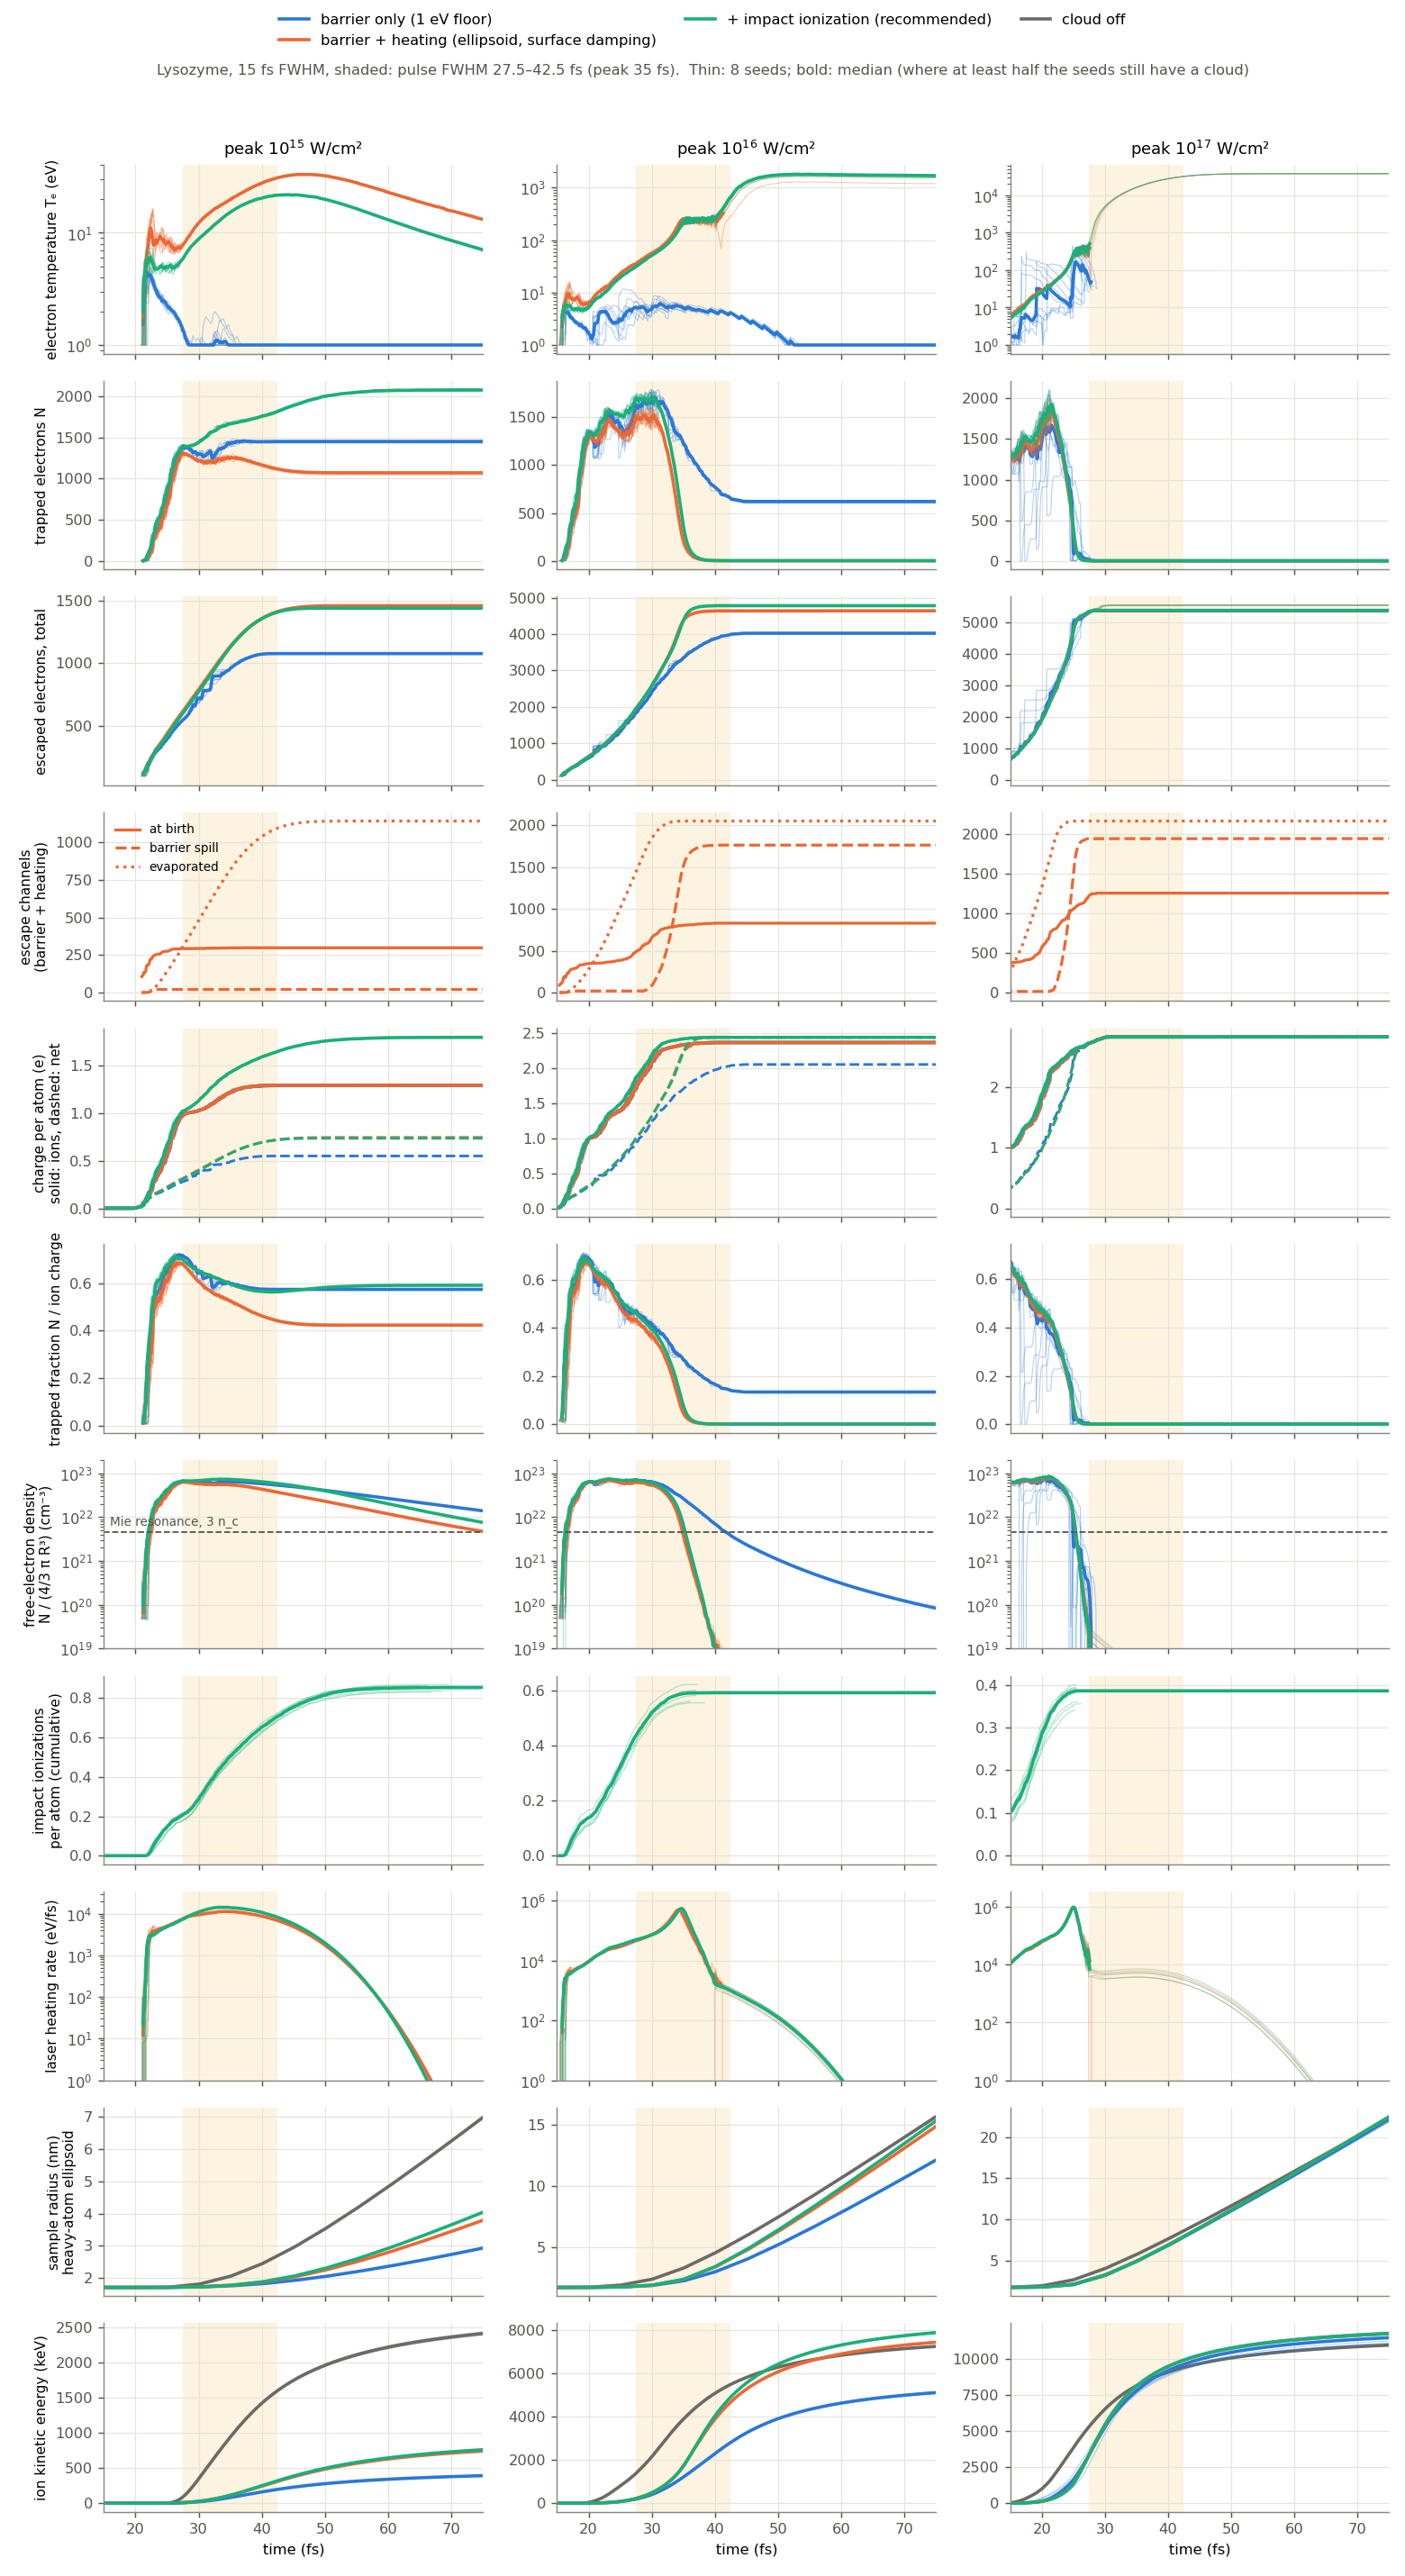
\includegraphics[width=0.92\textwidth]{fig/timeseries.png}
  \caption{The cloud over time, lysozyme, 8 seeds (thin) and their median (bold), for the current model built up step
  by step --- the barrier alone, with heating (ellipsoid, surface damping), and the recommended model with impact
  ionization --- against the cloud off; all with the 1\,eV temperature floor, 75\,fs (scan of 13 November 2026,
  build ref-pb17). With surface damping the heating passes the Mie resonance as a smooth maximum near the pulse peak;
  the earlier scan without it had 15--19\,MeV spikes in about 1 of 8 runs.}
  \label{fig:timeseries}
\end{figure}

\section{What the cloud does}

\begin{table}[H]
\centering\small
\begin{tabularx}{\textwidth}{@{}l X X X@{}}
\toprule
peak [W/cm$^2$] & trapped at the end & ion energy vs cloud off & direction shift vs cloud off (fast 25\,\% / all) \\
\midrule
$10^{15}$ & 59\,\% of the electrons & 0.32 & 8.7$^\circ$ / 13.9$^\circ$ \\
$10^{16}$ & 0 (gone by $\sim$45\,fs) & 1.09 & 3.7$^\circ$ / 5.7$^\circ$ \\
$10^{17}$ & 0 (gone by $\sim$28\,fs) & 1.07 & 3.4$^\circ$ / 5.1$^\circ$ \\
\bottomrule
\end{tabularx}
\caption{The cloud's effect in the recommended model (barrier, heating with the ellipsoid and surface damping, impact
ionization, 1\,eV floor; ref-pb17, 8 seeds, 75\,fs) against the cloud off. The seed spread of the fast ions' directions
(half against half) is 0.6--2.3$^\circ$, so the shifts are systematic. An earlier scan without surface damping, the
ellipsoid and the floor gave 47\,\% trapped, 0.31 and 6.5$^\circ$/8.7$^\circ$ at $10^{15}$, 1.01 and 3.4$^\circ$/4.7$^\circ$
at $10^{16}$.}
\end{table}
At $10^{17}$\,W/cm$^2$ the cloud leaves before the peak, but it holds the sample compact while ADK charges it, which gives
the ions about 7\,\% more energy than without it.

\section{Each option}

\begin{longtable}{@{}p{0.28\textwidth}p{0.66\textwidth}@{}}
\toprule
option & effect on lysozyme \\
\midrule
\endhead
field-free cloud & traps $\sim$98\,\% of the electrons at every intensity: wrong at high intensity \\
barrier, no heating & the cloud cools to the 1\,eV floor; at $10^{15}$ seed-bistable (1196 $\pm$ 436 trapped, ion energy
  701 $\pm$ 541\,keV) \\
heating & reproducible (1139 $\pm$ 9 trapped, 666 $\pm$ 2\,keV at $10^{15}$); at $10^{16}$ the trapped fraction drops from
  13\,\% to 1\,\% \\
collision-rate cap & 1 and no cap agree; 0.1 heats less (1393 trapped at $10^{15}$); 0.5 with the full model: $-16$\,\%
  heating and $-8$\,\% ion energy at $10^{15}$, nothing at $10^{16}$; directions unchanged \\
ellipsoid shape & $+13$\,\% heating, $+6$\,\% ion energy at $10^{15}$; $\sim$1\,\% at $10^{16}$; directions within noise \\
surface damping ($A=1$) & removes the resonance outliers (15--19\,MeV in 1 of 8 runs); seed spread of the ion energy at
  $10^{16}$ $\pm$90 $\to$ $\pm$28\,keV; ion energy $+2.5$\,\% ($10^{15}$), $+7$\,\% ($10^{16}$), $+1.6$\,\% ($10^{17}$);
  $A$ = 0.5 / 1 / 2: 7806 / 7912 / 7986\,keV at $10^{16}$ \\
barrier mode 2 & same charges, energies (within 2\,\%) and directions as mode 1; clamped energy in 3 of 24 runs \\
impact ionization & ion charge 1.29 $\to$ 1.72 per atom at $10^{15}$, +2.5\,\% at $10^{16}$; net charge and directions
  unchanged, ion energy $+6$\,\% ($10^{15}$) \\
recombination 2 & gives the charge back after the pulse (1.72 $\to$ 1.35), explosion unchanged \\
recombination 1 & capture--ADK pump: ADK events 1868 $\to$ 17\,284, ion energy $+22$\,\% \\
temperature floor 1\,eV & acts $\sim$0.02\,fs per run; ion energy 927 $\to$ 927\,keV ($10^{15}$), 7912 $\to$ 7901\,keV
  ($10^{16}$); removes the clamp \\
long range, 2\,nm & ion energy $+0.6$\,\%, directions within noise, force error 1\,\% rms ($10^{16}$, one seed) \\
\bottomrule
\end{longtable}

\section{The direction autostop and the schedule}
\label{sec:val-schedule}

Recommended model with the 1\,eV floor, 8 seeds, each run to 300\,fs and compared with the same seed stopped or
scheduled (identical up to the stop or the first change):

\begin{table}[H]
\centering\small
\begin{tabularx}{\textwidth}{@{}X l l@{}}
\toprule
 & $10^{15}$\,W/cm$^2$ & $10^{16}$\,W/cm$^2$ \\
\midrule
autostop 2: stop time & 125--130\,fs & 95\,fs (the earliest allowed) \\
turn after the stop to 300\,fs, fast 25\,\% / all & 0.87 / 2.17$^\circ$ & 0.40 / 0.56$^\circ$ \\
seed-to-seed spread at 300\,fs & 2.96 / 5.39$^\circ$ & 0.95 / 1.52$^\circ$ \\
ion energy at the stop vs 300\,fs & $-6.3$\,\% & $-6.1$\,\% \\
wall time, stop vs 300\,fs & 2.5$\times$ less & 3.3$\times$ less \\
\midrule
schedule (below) vs none at 300\,fs & 0.09 / 1.18$^\circ$ & 0.02 / 0.02$^\circ$ \\
schedule: ion energy & $-0.20$\,\% & $-0.03$\,\% \\
schedule: wall time & 2.8$\times$ faster & 3.1$\times$ faster \\
\bottomrule
\end{tabularx}
\end{table}
The schedule is \code{65:0.01:0.2 95:0.1:2 135:0.1:5}.
At $10^{16}$ the cloud is gone before the first change, so only the step changes; at $10^{15}$ the cloud is solved every
2--5\,fs late in the run, which moves the slow ions' directions by about 1$^\circ$, far below the spread.

\section{Linear polarization}
\label{sec:val-polarization}

\opt{sfmd-laser-polarization} (Section~\ref{sec:polarization}), build ref-pb18, against the same model without it
(the recommended defaults, no recombination), 8 seeds, 75\,fs. Lysozyme's gyration axes lie along the lab axes:
$x$ the long one (2.37\,nm), $y$ (1.51\,nm), $z$ the short one (1.38\,nm), so polarization along $x$, $y$ and $z$ is
the same protein in three orientations to the field. The unpolarized explosion is itself anisotropic in these axes
(it is slower along the long axis), so every anisotropy is compared along the same axis.

\begin{description}
  \item[The energy ledger.] A seeded cloud of 4000 electrons (no new electrons, no heating), $10^{15}$\,W/cm$^2$ for
    10\,fs: the polarized cloud's kinetic energy follows the direction-free one within 1\,\% through the run (end
    T = 4.65 against 4.26\,eV; 4.58\,eV with solves every 0.1\,fs). No numerical heating from the field.
  \item[Ion energy] (polarized against unpolarized):
    $10^{15}$: $x$ +6\,\%, $y$ $-18$\,\%, $z$ $-22$\,\% ($-22$\,\% also at 200\,fs);
    $3\times10^{15}$: $z$ $-37$\,\%; $10^{16}$: +1, $-5$, $-5$\,\%; $3\times10^{16}$: $z$ $-5$\,\%;
    $10^{17}$: $-1$, $-3$, $-5$\,\%. At low intensity this follows the heating, which depends on the axis through the
    depolarization factor ($10^{15}$: 368, 184, 160\,keV against 245 orientation-averaged; their mean, 237\,keV,
    matches the average); the ion energy averaged over the three orientations is still 12\,\% lower at $10^{15}$.
  \item[Escape] goes more by spilling and less by evaporation (at $10^{16}$ spilled 2370--2640 against 1750,
    evaporated 1550--1790 against 2200); the final charge is the same within 2\,\% from $10^{16}$ up and 10--12\,\%
    lower at $10^{15}$ along $y$ and $z$ (less heating, fewer impact ionizations).
  \item[Shape.] The heavy-ion velocities are elongated along the polarization: $\langle v_a^2\rangle/\langle
    v_\perp^2\rangle$ rises by 0.015--0.04 at $3\times10^{15}$ and above (seed spread 0.002--0.005), e.g.\ $z$ at
    $10^{16}$ 1.114 against 1.080. At $10^{15}$ along $x$ it falls by 0.05: there the cloud stays (60\,\% trapped)
    and its pressure pushes the elongated protein out along its short axes, the more so the hotter it is (ratio along
    $x$: 1.14 without heating, 0.85 with 245\,keV, 0.80 with polarization $x$ and 368\,keV), which outweighs the
    field's stretch; compared at similar heating, $y$ and $z$ show the stretch, +0.03--0.05. From $10^{16}$ up the
    cloud is gone by 45\,fs and only the stretch remains. The charge of the ions near the poles against the equator
    does not change beyond the seed spread.
  \item[Directions.] The seed-averaged directions move by 1.8--2.1$^\circ$ (fast quarter) at $10^{15}$ and
    0.7--1.0$^\circ$ from $10^{16}$ up, against 1.4--1.5$^\circ$ and 0.4--0.6$^\circ$ expected from seed noise alone
    (two 8-seed means differ by about half the root-sum-square of the half-against-half angles): a systematic shift
    of 0.5--1$^\circ$, a fifth or less of what the cloud itself does (3--6.5$^\circ$).
  \item[Solve interval.] At $10^{16}$ along $z$, solves every 0.1\,fs instead of 0.2\,fs give the same ion energy
    (7491 against 7483\,keV), charge, elongation (1.115 against 1.114) and polarization work, and directions within
    the seed noise (0.6$^\circ$); only the split between spilling and evaporation moves (spilled 2254 against 2583),
    since spills happen at the solves.
  \item[The box.] Weighted by the trapped electrons, the adaptive box leaves at most 0.5\,\% of the cloud outside
    (0.03\,\% without the polarization; the target is 2\,\%).
  \item[The escape-level fix.] The first version (ref-pb17) took, when no saddle lies outside the sample, a level
    deep inside it; along the long axis a neutral cloud was then held at $10^{17}$\,W/cm$^2$ (130\,MeV heating in 1
    of 8 runs). All numbers above are from the fixed version (ref-pb18).
\end{description}

\section{What is not tested}

\begin{itemize}
  \item Other systems, sizes, wavelengths and pulse lengths; samples above 10\,000 atoms (long range, its speed-up).
  \item Comparison with experiment or with an explicit-electron code.
  \item Intensities below $10^{15}$ or above $10^{17}$\,W/cm$^2$; the run summary warns outside that range.
\end{itemize}

\chapter{Versions, tests and limitations}
\label{app:misc}

\section{File format versions}

The \file{.tpr} carries the \opt{sfmd-*} options.
Stock GROMACS 4.5.4 writes version 73; this build writes 185 and reads stock files.
It refuses 74 and 76--174, which \code{gromacs-mc} uses for a different layout, instead of misreading them.

\begin{table}[H]
\centering\small
\begin{tabular}{@{}l l@{}}
\toprule
version & added \\
\midrule
75 & the strong-field options (pulse, autostop, initial charges, output) \\
175 & the trapped-electron cloud (\opt{sfmd-electrons}, \opt{sfmd-pb-*}, \opt{sfmd-evaporation}) \\
176 & \opt{sfmd-laser-barrier} \\
177 & \opt{sfmd-laser-heating}, \opt{sfmd-heating-nu-cap} \\
178 & \opt{sfmd-collisions} \\
179 & \opt{sfmd-coll-recombination} \\
180 & \opt{sfmd-heating-shape} \\
181 & \opt{sfmd-heating-surface} \\
182 & \opt{sfmd-te-min} \\
183 & \opt{sfmd-autostop = 2} and its \opt{-angle}, \opt{-interval}, \opt{-min-time} \\
184 & \opt{sfmd-schedule} \\
185 & \opt{sfmd-laser-polarization} \\
\bottomrule
\end{tabular}
\end{table}
An older \file{.tpr} reads with each newer option at the value that keeps its behaviour (off, or the old model).

\section{Renamed and removed options}

\code{grompp} refuses these and names the replacement, because a warning would be swallowed by \code{-maxwarn} and
several changed meaning as well as name.

\begin{table}[H]
\centering\small
\begin{tabularx}{\textwidth}{@{}l X@{}}
\toprule
old & new \\
\midrule
\opt{sfmd-autostop-threshold} & \opt{sfmd-autostop-energy-ratio} (same value; renamed with autostop 2, as
  \code{gromacs-mc}) \\
\opt{sfmd-recombination} & \opt{sfmd-coll-recombination} (same values, \code{gromacs-mc}'s name) \\
\code{userint1} & removed: \code{-ionize} alone enables the modified force field \\
\code{userint2}, \code{userint4}, \code{userint6} & removed (never read by this build) \\
\code{userint3}, \code{userint5}, \code{userint9} & \opt{sfmd-autostop}, \opt{sfmd-detailed-output},
  \opt{sfmd-initial-charges} \\
\code{userint7} & \opt{sfmd-charge-output-stride} --- not the same: it writes every $N$th step \\
\code{userreal1} & \opt{sfmd-pulse-peak-time}, now in fs (multiply by 1000) \\
\code{userreal2}, \code{userreal4}, \code{userreal5} & \opt{sfmd-pulse-energy}, \opt{sfmd-pulse-focal-diameter},
  \opt{sfmd-pulse-wavelength} \\
\code{userreal3} & \opt{sfmd-pulse-fwhm}, now the FWHM in fs (was $\sigma$ in ps: multiply by 2354.82) \\
\code{userreal6} & \opt{sfmd-autostop-energy-ratio} \\
\bottomrule
\end{tabularx}
\end{table}

\section{Tests}

\begin{description}
  \item[\file{test/invariance.sh}] 23 short cases (water and lysozyme, one and four ranks, both stops, the schedule,
    fixed charges, and each cloud option in turn, the defaults, long range and the polarization), compared bit for bit with checksums from
    a frozen build (machine-specific; \code{--ref-bindir} compares two builds directly).
    Each case also checks what holds on any build: events against charges, no clamped cloud energy, escaped plus
    trapped equal to the events, that the option under test acted.
    Every change to the code has to pass it, and a change that adds an option must leave every earlier case
    unchanged.
  \item[\file{test/regression.sh}] the original water-cluster check of event counts and charges.
  \item[\file{test/pb\_vs\_mc.sh}] the field-free cloud against \code{gromacs-mc}, bit for bit (needs a
    \code{gromacs-mc} build with \file{test/mc\_pb\_seed.patch}).
\end{description}

\section{Limitations}

\begin{itemize}
  \item \textbf{Valence shell only} (Table~\ref{tab:adk}); elements without ADK data stay neutral.
  \item \textbf{ADK}: the tunnelling limit, from the ground state, without the local field of neighbours and cloud.
  \item \textbf{The laser has no direction} by default: the barrier is lowered all round, the heating is
    orientation-averaged. \opt{sfmd-laser-polarization} (development) puts the field along one axis into the solve;
    there is no quiver or drift motion of single electrons either way.
  \item \textbf{One temperature}, a Maxwellian cloud in instantaneous equilibrium; the least reliable late at
    $10^{15}$\,W/cm$^2$, where the cloud cools towards the floor.
  \item \textbf{Not fitted}: the collision-rate cap and the surface-damping constant are order-of-magnitude choices; their
    sensitivity is in Appendix~\ref{app:validation}.
  \item \textbf{No restart with the cloud}: its state is not saved, and \opt{sfmd-initial-charges} is refused with it.
  \item \textbf{Numerical stability}: very high charges give large forces; if the energies are not smooth, lower the step.
  \item Tested on Linux only.
\end{itemize}


\begin{thebibliography}{99}
\small
\bibitem{pronk2013} S.~Pronk \emph{et al.}, \emph{GROMACS 4.5: a high-throughput and highly parallel open source
molecular simulation toolkit}, Bioinformatics \textbf{29}, 845 (2013).
\bibitem{adk1986} M.~V.~Ammosov, N.~B.~Delone, V.~P.~Krainov, \emph{Tunnel ionization of complex atoms and of atomic
ions in an alternating electromagnetic field}, Sov.\ Phys.\ JETP \textbf{64}, 1191 (1986).
\bibitem{tong2002} X.~M.~Tong, Z.~X.~Zhao, C.~D.~Lin, \emph{Theory of molecular tunneling ionization}, Phys.\ Rev.\ A
\textbf{66}, 033402 (2002).
\bibitem{lotz1968} W.~Lotz, \emph{Electron-impact ionization cross-sections and ionization rate coefficients for atoms
and ions from hydrogen to calcium}, Z.\ Phys.\ \textbf{216}, 241 (1968).
\bibitem{ditmire1996} T.~Ditmire, T.~D.~Donnelly, A.~M.~Rubenchik, R.~W.~Falcone, M.~D.~Perry, \emph{Interaction of
intense laser pulses with atomic clusters}, Phys.\ Rev.\ A \textbf{53}, 3379 (1996).
\bibitem{saalmann2006} U.~Saalmann, Ch.~Siedschlag, J.~M.~Rost, \emph{Mechanisms of cluster ionization in strong laser
pulses}, J.\ Phys.\ B \textbf{39}, R39 (2006).
\bibitem{fennel2010} Th.~Fennel \emph{et al.}, \emph{Laser-driven nonlinear cluster dynamics}, Rev.\ Mod.\ Phys.\
\textbf{82}, 1793 (2010).
\bibitem{kreibig1995} U.~Kreibig, M.~Vollmer, \emph{Optical Properties of Metal Clusters} (Springer, 1995).
\bibitem{chen2016} F.~F.~Chen, \emph{Introduction to Plasma Physics and Controlled Fusion}, 3rd ed.\ (Springer, 2016).
\bibitem{nrl} J.~D.~Huba, \emph{NRL Plasma Formulary} (Naval Research Laboratory, revised editions).
\bibitem{mermin1965} N.~D.~Mermin, \emph{Thermal properties of the inhomogeneous electron gas}, Phys.\ Rev.\
\textbf{137}, A1441 (1965).
\bibitem{darden1993} T.~Darden, D.~York, L.~Pedersen, \emph{Particle mesh Ewald: An N$\cdot$log(N) method for Ewald sums
in large systems}, J.\ Chem.\ Phys.\ \textbf{98}, 10089 (1993).
\bibitem{essmann1995} U.~Essmann \emph{et al.}, \emph{A smooth particle mesh Ewald method}, J.\ Chem.\ Phys.\
\textbf{103}, 8577 (1995).
\bibitem{abramowitz1964} M.~Abramowitz, I.~A.~Stegun, \emph{Handbook of Mathematical Functions} (NBS, 1964), ch.~6.
\bibitem{birdsall1991} C.~K.~Birdsall, A.~B.~Langdon, \emph{Plasma Physics via Computer Simulation} (IOP, 1991).
\bibitem{hockney1988} R.~W.~Hockney, J.~W.~Eastwood, \emph{Computer Simulation Using Particles} (Adam Hilger, 1988).
\bibitem{hockney1970} R.~W.~Hockney, \emph{The potential calculation and some applications}, Methods Comput.\ Phys.\
\textbf{9}, 135 (1970).
\bibitem{eastwood1979} J.~W.~Eastwood, D.~R.~K.~Brownrigg, \emph{Remarks on the solution of Poisson's equation for
isolated systems}, J.\ Comput.\ Phys.\ \textbf{32}, 24 (1979).
\bibitem{frigo2005} M.~Frigo, S.~G.~Johnson, \emph{The design and implementation of FFTW3}, Proc.\ IEEE \textbf{93},
216 (2005).
\bibitem{nocedal2006} J.~Nocedal, S.~J.~Wright, \emph{Numerical Optimization}, 2nd ed.\ (Springer, 2006).
\bibitem{gould2001} N.~I.~M.~Gould, M.~E.~Hribar, J.~Nocedal, \emph{On the solution of equality constrained quadratic
programming problems arising in optimization}, SIAM J.\ Sci.\ Comput.\ \textbf{23}, 1376 (2001).
\end{thebibliography}

\end{document}
